\documentclass[a4paper]{report}
\usepackage[utf8]{inputenc}
\usepackage{amssymb}
\usepackage[ngerman]{babel}
\usepackage{hyperref}
\usepackage{enumitem}
\usepackage{listings}
\usepackage{esvect}
\usepackage{float}
\usepackage{graphicx}
\usepackage{todonotes}
\usepackage{pgfplots}
\usepackage{verbatim}
\pgfplotsset{compat=1.10}
\usepgfplotslibrary{fillbetween}
\usetikzlibrary{patterns}
\usepackage{mathtools}
\usepackage{centernot}

\hypersetup{
     colorlinks   = true,
     citecolor    = gray
}

%https://www.google.com/search?q=latex+math+symbols&oq=latex+math+&aqs=chrome.0.69i59j69i57j69i61j69i60l2j35i39.2187j0j7&sourceid=chrome&ie=UTF-8

%||norm||
\newcommand{\norm}[1]{\left\lVert#1\right\rVert}
%Skalarprodukt <.,.>
\newcommand{\dotProduct}[2]{\langle#1,#2\rangle}

%\emph -> fettgedruckt
\let\emph\relax
\DeclareTextFontCommand{\emph}{\bfseries}

% Paragraph, wobei der Text in neuer Zeile ohne indent beginnt
\newcommand{\newlinepar}[1]{\paragraph{#1}\mbox{}\\\noindent}

%\emph -> fettgedruckt
\let\emph\relax
\DeclareTextFontCommand{\emph}{\bfseries}

% d in integralen
\newcommand*\diff{\mathop{}\!\mathrm{d}}
\newcommand*\Diff[1]{\mathop{}\!\mathrm{d^#1}}

% Residue
\newcommand{\res}{\text{Res}}

% f im Text
\newcommand{\f}{$f$ }



% Spaltenvektor der Länge n
% geklaut von https://tex.stackexchange.com/questions/2705/typesetting-column-vector
\newcount\colveccount
\newcommand*\colvec[1]{
        \global\colveccount#1
        \begin{pmatrix}
        \colvecnext
}
\def\colvecnext#1{
        #1
        \global\advance\colveccount-1
        \ifnum\colveccount>0
                \\
                \expandafter\colvecnext
        \else
                \end{pmatrix}
        \fi
}

% Ableitung eines Vektors
\def\vecderiv#1{\vec#1\,'}

% Small vectors (inline) https://tex.stackexchange.com/a/200511/143051
\newcommand{\smallcolvec}[1]{% inline column vector
  \left(\begin{smallmatrix}#1\end{smallmatrix}\right)%
}
\newcommand{\smallrowvec}[1]{% inline row vector
  \begin{smallmatrix}(#1)\end{smallmatrix}%
}

\begin{document}
\begin{titlepage}
    \centering
    \vfill
    
\includegraphics[width=13cm]{UniUlmLogo.PNG} % also works with logo.pdf
    \vfill
    \vfill
    {\bfseries\Large
        Zusammenfassung Höhere Mathematik für Physiker \& Ingenieure 2/3\\
        WS18/19\\
    }    
    \vskip2cm
        Jonas Otto\\ \href{mailto:edwin.otto@uni-ulm.de}{edwin.otto@uni-ulm.de}\\
        Luca Krüger\\ \href{luca.krueger@uni-ulm.de}{luca.krueger@uni-ulm.de}\\
        Marco Deuscher\\ \href{marco.deuscher@uni-ulm.de}{marco.deuscher@uni-ulm.de}\\
        Simon Wilhelmstätter\\ \href{simon.wilhelmstaetter@uni-ulm.de}{simon.wilhelmstaetter@uni-ulm.de}\\
        \vfill
     März 2019
    \vfill
    \vfill
    \vfill
\end{titlepage}

\clearpage

%\maketitle

%\listoftodos
%\newpage

\tableofcontents
\newpage

\section*{Disclaimer}
Mit dem Bearbeiten dieses Dokuments verpflichtet sich der Autor, allen oben aufgeführten anderen Autoren ein (1) Bier auszugeben, falls die hinzugefügten Informationen offensichtlich falsch sind, richtiges oder relevantes entfernt oder das Dokument in anderer Weise negativ/destruktiv beeinflusst wurde.


\begin{comment}

\section*{Notizen/Anmerkungen}
\paragraph{Bemerkungen von Liebezeit in letzter Vorlesung}
\begin{enumerate}
    \item Aufgabe 42 (Jordansches Lemma anschauen)
    \item Eine Aufgabe hat wahrscheinlich eine nicht endliche Anzahl an Singularitäten(Häufungspunkt). Residuensatz kann an dieser Stelle nicht angewendet werden. Es sollte aber möglich sein das Integral mittels passender Integrationswege zu bestimmen. (Halbkreise)
\end{enumerate}

\end{comment}


\chapter{Lineare Algebra}
\section{Matrizen}
\subsection{Hermitesche Matrizen}
\begin{itemize}
    \item $\iff A^H = A$
    \item $\implies$ Eigenwerte $\lambda_i \in \mathbb{R}$
    \item $\implies A$ normal
    \item $\implies$ unitär diagonalisierbar. 
\end{itemize}

\subsection{Invertierbare/Reguläre Matrizen}
\begin{itemize}
    \item $\iff \det{A} \neq 0$ 
\end{itemize}

\subsection{Unitäre Matrizen}
\begin{itemize}
    \item $\iff A^H = A^{-1}$
    \item $\implies A$ regulär ($\iff$ invertierbar)
    \item $\implies |\det{A}| = 1$
    \item $\implies A$ normal
    \item $\implies$ Eigenvektoren orthonormal
\end{itemize} 

\subsection{Normale Matrizen}
\begin{itemize}
    \item $\iff A^H A = A A^H$
    \item $\iff A$ unitär diagonalisierbar
\end{itemize}

\subsection{Diagonalisierbare Matrizen}
\begin{itemize}
    \item $\iff S^{-1}AS = D$, $D$ Diagonalmatrix
\end{itemize}
\subsubsection{Diagonalisierbarkeit zeigen}
\begin{itemize}
    \item Charakteristisches Polynom zerfällt in Linearfaktoren
    \item $\wedge$ Geometrische und Algebraische Vielfachheiten stimmen überein
\end{itemize}

\subsubsection{Unitär Diagonalisierbare Matrizen}
\begin{itemize}
    \item $\iff \exists S$ unitär $\mid S^H=S^{-1}$
    \item $\implies$ Eigenvektoren orthogonal
\end{itemize}

\subsection{Spur einer Matrix}
Die Spur einer Matrix A ist die Summe der Hauptdiagonalelemente\\ $\sum\nolimits_{i=1}^n a_{ii} = Spur(A)$.
\begin{itemize}
    \item bei diagonalisierbaren Matrizen ist die Spur die Summe der Eigenwerte $\implies$ die Spur ähnlicher Matrizen ist gleich
    \item die Spur ist eine lineare Abbildung
    \item Vertauschung unter der Spur: $Spur(AB)=Spur(BA)$
    \item Invarianz bei zyklischen Vertauschungen $Spur(ABC)=Spur(BCA)=Spur(CAB)$
\end{itemize}

\subsection{Diagonalisieren von Matrizen}
Matrix $A$ diagonalisierbar $\iff D_A=S^{-1}AS$, $A=SDS^{-1}$. Es sollen $D_A$ und $S$ berechnet werden.
\begin{enumerate}
    \item Bestimmen der Eigenwerte $\lambda_i$ mittels $\det(A-\lambda I) = 0$.
    \item Bestimmen der Eigenräume $E(\lambda_i)$ zu den Eigenwerten mittels $(A-\lambda_iI)\cdot x = 0$
    \item Bestimmen der Basisvektoren $b$ der Eigenräume
    \item $D_A = \text{diag}(\lambda_1,\dots , \lambda_n)$\\ $S=(b_1,\dots,b_n)$
\end{enumerate}

\subsection{Definitheit}
Wenn eine Matrix nicht symmetrisch oder hermitesch ist, kann nur der symmetrische oder
hermitesche Teil betrachtet werden: $A_S=\frac{1}{2} (A+A^T)$ bzw $A_H=\frac{1}{2}(A+A^H)$.

\subsubsection{Definition}
Eine Matrix ist genau dann\\
\begin{tabular}{l l}
    positiv definit,	    &falls $x^{T}Ax>0$\\
    positiv semidefinit,	&falls  $x^{T}Ax\geq 0$\\
    negativ definit,	    &falls  $x^{T}Ax<0$\\
    negativ semidefinit,	&falls  $x^{T}Ax\leq 0$.
\end{tabular}

\subsubsection{Definitheit anhand von Eigenwerten}
Eine Matrix ist genau dann\\
\begin{tabular}{l l}
    positiv definit,        &wenn alle Eigenwerte größer als null sind;\\
    positiv semidefinit,	&wenn alle Eigenwerte größer oder gleich null sind;\\
    negativ definit,        &wenn alle Eigenwerte kleiner als null sind;\\
    negativ semidefinit,	&wenn alle Eigenwerte kleiner oder gleich null sind;\\
    indefinit,	            &wenn positive und negative Eigenwerte existieren.
\end{tabular}

\subsubsection{Definitheit anhand von Hauptminoren}
Positiv definit: Führende Hauptminoren sind positiv\\
Negativ definit: Vorzeichen der führenden Hauptminoren alternieren
(ungerade führende Hauptminoren negativ, alle geraden positiv).

\subsection{Satz von Cayley-Hamilton}
Matrix ist Nullstelle des Zugehörigen charakteristischen Polynoms:\\
$P_A(A) = (-1)^n(A^n + a_{n-1}A^{n-1}+\dots+a_0E_n)=0$\\
Durch Multiplizieren von $A^{-1}$ lässt sich damit $A^{-1}$ bestimmen.

% \section{Hauptachsentransformation}
% WORK IN PROGRESS/PLEASE FIX
% Gegeben sei Eine Quadrik $Q(x)=x^TAx+b^Tx+c=0$.
% Eventuell müssen die Matrizen noch aus einer gegebenen Gleichung aufgestellt werden.

% \begin{enumerate}
%     \item Bestimmen der Eigenwerte $\lambda_i$ von $A$ mittels $\det(A-\lambda I) = 0$.
%     \item Bestimmen der Eigenvektoren $e_i$ mit $(A-\lambda_i)\cdot e_i=0$ und anschließendem Normieren.
%     \item Aufstellen der Matrix $S=(e_1,\dots,e_n)$
%     \item Substituieren von $x,y,z$ durch $\widetilde{x},\widetilde{y},\widetilde{z}$ mit $(x,y,z)^T=S \cdot (\widetilde{x},\widetilde{y},\widetilde{z})^T$
% \end{enumerate}

\section{Determinanten}
\subsection{Umfomungen von Determinanten}
\begin{enumerate}
    \item \emph{Vertauschen} von Zeile oder Spalte $\implies$ Faktor $-1$ vor Determinante
    \item \emph{Multiplizieren} von Zeile $\implies$ Faktor vor Determinante
    \item \emph{Gauß} ohne Folgen
    \item $\det(A^{-1})=(\det(A))^{-1}$
\end{enumerate}

\section{Basiswechsel}
Ein VR zur Basis $A$ soll durch die Transformationsmatrix in die Basis $B$ umgeformt werden.
Berechnung der Trafomatrix mittels Gauß-Jodan:\\
$(B\mid A) \text{(Umformungen mit Gauß)} \implies  (E\mid T)$ \\ mit $E$ als Einheitsmatrix und $T$ als Tranformationsmatrix.
\subsection{Lineare Abbildung nach Basiswechsel}

Wichtig: Transformationsschritte links anmultiplizieren.

\begin{figure}[H]
    \centering
    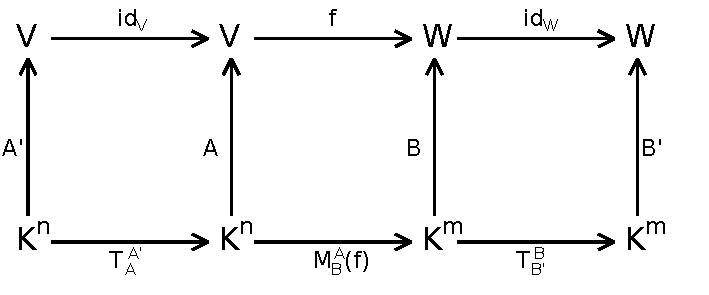
\includegraphics[width=0.8\textwidth]{Change_of_basis2.pdf}
    \caption{Basiswechsel linearer Abbildungen}
\end{figure}

In den meisten Fällen gilt bei uns $A=B$ und $ A'=B'$ und somit $T_{B'}^{B}$ invers zu $T_A^{A'}$. 

\section{Skalarprodukte}
Ein Skalarprodukt ist gegeben durch $f(x,y)= _{\dots} =x^T My$
\begin{enumerate}
    \item $\iff M$ hermitesch $\wedge$ $M$ positiv definit $\wedge$ M linear.
\end{enumerate}

\section{Lineare Abbildungen}
\subsection{Linearität zeigen}
\begin{itemize}
    \item Abbildung als Matrix darstellen
    \item $\alpha Lv = L(\alpha v) \wedge Lv_1 + Lv_2 = L(v_1+v_2)$
\end{itemize}

\subsection{Linearität widerlegen}
\begin{itemize}
    \item Additivität widerlegen: $Lv_1 + Lv_2 \neq L(v_1+v_2)$
    \item Abbildung auf Null widerlegen: $L0 \neq 0$
    \item Skalarmultiplikation widerlegen: $\alpha L v_1 \neq L(\alpha v_1)$
\end{itemize}


\section{Gram Schmidt}
\begin{enumerate}
    \item $u_1 = \frac{v_1}{\norm{v_1}}$
    \item $u_2^\prime = v_2 - \langle v_2,u_1 \rangle u_1$
    \item $u_2 = \frac{u_2^\prime}{\norm{u_2^\prime}}$
    \item $u_k^\prime = v_k - \sum_{i=1}^{k-1}\langle v_k,u_i\rangle u_i$
    \item $u_k = \frac{u_k^\prime}{\norm{u_k^\prime}}$
\end{enumerate}

\section{Vektorräume}
\subsection{Voraussetzungen}
\begin{itemize}
    \item $V \neq \varnothing$
    \item $(V,+)$ abelsche Gruppe (kommutative Vektoraddition)
        \begin{itemize}
            \item Assoziativität, Neutrales, Inverses, Kommutativität
        \end{itemize}
    \item \emph{Vektorraumaxiome}
        \begin{itemize}
            \item $1 \cdot v = v$
                \item $(\lambda + \mu)\cdot v = \lambda v + \mu v$,  $\lambda (v + w) = \lambda v + \lambda w$ Distributivgesetzt bzgl. Skalarmultiplikation, Vektoraddition
            \item  $\lambda (\mu v) = (\lambda \cdot \mu) \cdot v$ Assoziativgesetz
        \end{itemize}
\end{itemize}

\subsection{Vektorraum zeigen}
Einfacher als Axiome: \emph{Unterraumkriterium}:
\begin{itemize}
    \item Abgeschlossenheit bzgl. Vektoraddition
    \item Abgeschlossenheit bzgl. Skalarmultiplikation
\end{itemize}

\chapter{Funktionen mehrerer Veränderlicher}
\section{Topologie}
\subsection{Grundbegriffe}
Sei $(M,d)$ ein metrischer Raum $\wedge \  A \subseteq M$,$a \in M$ dann ist:
\begin{itemize}
    \item  Inneres $\overset{\circ}{A} :=\{a\in M\ \vert \ \exists \ \varepsilon >0         :U_{\varepsilon}(a) \subseteq A\}$
    \item Abschluss $\overline{A}:=\{ a \in M\ \vert \ \forall \varepsilon>0 :               U_\varepsilon(a) \cap A \neq \varnothing \}$
    \item Häufungspunkt $A^\prime:=\{\forall \varepsilon>0 : \.{U}_\varepsilon(a) \cap A         \neq \varnothing \}$ 
    \item Randpunkte $\partial A:= \{a \in M\ \vert \ \forall \varepsilon>0\ \exists         x,y:x\in A , y\in A^c\ \wedge \ x,y \in U_\varepsilon(a) \}$
    \item Bedingung für Isolierte Punkte $a\in A:\ \ \exists \ \varepsilon>0 :               U_\varepsilon(a) \cap A =\{a\}$
    \item \underline{offene Menge}
    \subitem $\iff$ jedes $a\in A$ ist innerer Punkt von $A$ 
    \item \underline{abgeschlossene Menge}
    \subitem $\iff \ A^c$ ist offen 
    \subitem $\iff \partial A \subseteq A$ 
    \subitem $\iff A=\overline{A}$
    \item $K \subset \mathbb{R}$ kompakt $\iff K$ beschränkt und abgeschlossen
\end{itemize}

\subsection{Metriken}
Sei $X$ eine beliebige Menge, dann ist $d: X\times X \rightarrow \mathbb{R}$ eine Metrik wenn für $x,y,z\in X$ folgende Axiome erfüllt sind:
\begin{itemize}
    \item [(M$1$)] Pos. Definitheit $d(x,y)\ge 0 \ \wedge \ d(x,y)=0 \iff x=y$
    \item [(M$2$)] $d(x,y)=d(y,x)$
    \item [(M$3$)] Dreiecksungleichung $d(x,y)\le d(x,z)+d(z,y)$
\end{itemize}

\section{Funktionen und Abbildungen}


\section{Differenzierbarkeit}
\subsection{Grundbegriffe}
\begin{itemize}
    \item partielle Ableitung:\\ $\frac{\partial f}{\partial x_j}(x_0) = d_j f(x_0) = \lim_{h\to 0}\frac{f(x_1^{(0)} \dots x_j^{(0)}+h \dots x_n^{(0)})-f(x_0)}{h}$\\
    f ist partiell diff'bar in $x_0$ falls alle partiellen Ableitungen existieren mit $\nabla f(x_0)$
    \item Stetigkeit in Achsenrichtung: \\
    Ist f in $x_0$ nach $x_i$ diff'bar, so ist f in $x_0$ in Richtung der $x_i$-Achse stetig. ($\neq$ Stetigkeit in alle Richtungen)
    \item Richtungsableitungen:\\
    $e \in \mathbb{R}^n$ ein Richtungsvektor mit $\norm{e}=1$, $x_0 \in U$ existiert \\
    $\lim_{h\to 0}\frac{f(x_0 + he)-f(x_0)}{h}$, so ist dies die Richtungsableitung von f nach $e$ in $x_0$: $\frac{\partial f}{\partial e}(x_0)$\\
    Der Gradient ist ein Spezialfall einer Richtungsableitung und steht immer senkrecht auf den Höhenlinien ($f(x) = c$) und zeigt in die Richtung des stärksten Anstiegs.
\end{itemize}
\subsubsection{Totale Ableitung}
Eine Funktion $f: U\to \mathbb{R}^n$ ist in $x_0 \in U$ total diff'bar, falls f in $x_0$ linearisierbar ist: \\
\begin{equation}
    \bigvee x \in U \  \exists A: f(x) = f(x_0) + A(x-x_0) + r(x,x_0)
\end{equation}
wobei $A$ eine Matrix und $r(x,x_0)$ ein Restterm ist.\\
Bemerkung: $A$ ist die Jacobi-Matrix, bzw bei einer skalarwertigen Funktion der (transponierte) Gradient der Funktion an der entsprechenden Stelle.\\
Ist f in U partiell diff'bar und die partiellen Ableitungen in $x_0$ stetig, dann ist f total diff'bar.\\
Notation: $f'(x_0) = Df(x_0)$\\
Für den Restterm muss gelten 
\begin{equation}
    \lim_{x\to x_0}\frac{\|r(x,x_0)\|}{\|x-x_0\|} = 0
\end{equation}

\subsubsection{Totale Diff'barkeit und Richtungsableitungen}
Ist f in $x_0$ total diff'bar, dann ist f in $x_0$ in jede Richtung diff'bar und für die Richtungsableitungen gilt 
\begin{equation}
    \frac{\partial f}{\partial e} = \langle \nabla f(x_0),e\rangle = - \frac{\partial f}{\partial (-e)} = \lim_{h\to 0}\frac{f(x_0+he)-f(x_0)}{h}
\end{equation}
Beachte, aus Diff'barkeit in jede Richtung folgt nicht totale Diff'barkeit, sobald die partiellen Ableitungen nicht stetig sind!

\subsection{Mehrdimensionale Kettenregel}
Sind $f:\mathbb{R}^n\to \mathbb{R}^l$ und $g:\mathbb{R}^l\to \mathbb{R}^m$ diff'bare Abbildungen, dann ist auch $g\circ f: \ \mathbb{R}^n\to \mathbb{R}^m$ diff'bar. Die Ableitung im Punkt p ist dann als die Hintereinanderausführung der Ableitung von \f in p und der Ableitung von g in $f(p)$ definiert
\begin{equation}
    D(g\circ f)_p = Dg_{f(p)}\circ Df_p
\end{equation}

\noindent Wird die Verkettung mit $h(x)= g\circ f$ definiert gilt dann 
\begin{equation}
    \frac{\partial h_i}{\partial x_j}(p) = \sum_{k=1}^{l} \frac{\partial g_i}{\partial y_k}(f(p)) \cdot \frac{\partial f_k}{\partial x_j}(p)
\end{equation}
hierbei werdem die Koordinaten im Def-Bereich von f als $x=(x_1,\dots,x_n)$ und die Koordinaten im Bildraum $\mathbb{R}^l$ von \f mit $y=(y_1,\dots,y_l)$ bezeichnet.

\subsection{Satz von Schwarz}
Existiert die partielle Ableitung ist $\frac{\partial^2 f}{\partial x_j \partial x_i}(x_0)$ die zweite partielle Ableitung von f nach $x_i$ und $x_j$ (in dieser Reihenfolge).\\

Ist f in einer Umgebung von $x_0 \in \mathbb{R}^n$ stetig, existieren in $x_0$ $f_{x_i},f_{x_j},f_{x_i,x_j},f_{x_j,x_i}$ und sind die zweiten partiellen Ableitungen stetig in $x_0$ so gilt
\begin{equation}
    \frac{\partial^2 f}{\partial x_i \partial x_j} = \frac{\partial^2 f}{\partial x_j \partial x_i}
\end{equation}
Das ist gleichbedeutend damit, dass die Hesse-Matrix symmetrisch ist.

\section{Lokale Extrema}

\newlinepar{Vorgehensweise: Extrema im $\mathbb{R}^n$ bestimmen}
\begin{enumerate}
    \item Gradient $\nabla f(x)$ bestimmen
    \item $\nabla f(x) = 0$ lösen
    \item Hesse-Matrix betrachten um Art des Extremums zu bestimmen  (\nameref{subsec:zweite-ableitung-krit-hessematrix})
\end{enumerate}

\subsection{Satz von Fermat}
\begin{itemize}
    \item $U \subset \mathbb{R}$ offen
    \item $f$ besitze in $x_0 \in U $ ein lokales Extremum und dort partiell diff'bar \\
    $\Rightarrow \nabla f(x_0) = 0$ 
    \item gilt $\nabla f(x_0) = 0$ heißt $x_0$ kritischer oder stationärer Punkt von $f$ 
\end{itemize}

\subsection{Zweite Ableitung Kriterium}
\label{subsec:zweite-ableitung-krit-hessematrix}
Es sei $f \varepsilon C^2(U)$ und $x_0 \in U$ ist kritischer Punkt $\Rightarrow \nabla f(x_0) = 0$
\begin{itemize}
    \item Hesse-Matrix positiv definit $\Rightarrow$ Minimum
    \item Hesse-Matrix negativ definit $\Rightarrow$ Maximum
    \item Hesse-Matrix indefinit $\Rightarrow$ Sattelpunkt
    \item Hesse-Matrix semi-positiv definit $\Rightarrow$ Minimum oder Sattelpunkt
    \item Hesse-Matrix semi-negativ definit $\Rightarrow$ Maxiumum oder Sattelpunkt
    \item Hesse-Matrix semi definit $\Rightarrow$ keine Aussage möglich. Betrachtung mit Definition und ggf. $\varepsilon$-Umgebung
\end{itemize}

\section{Implizite Funktionen}
\subsection{Lokale Injektivität}
$f \in C^2(U,\mathbb{R}^n$), $a \in U$ und $\vert Jf(a)\vert \neq 0$. Dann ist f lokal injektiv: \\
Es gibt offene Umgebung $U(a) \subset U$, so dass f auf diese Umgebung eingeschränkt injektiv ist.

\subsection{Lemma 2.5.5}
Es sei $f \in C^1(U,\mathbb{R}^n)$ injektiv, $a \in U$ mit $b := f(a)$. b ist dann innerer Punkt von $f(U)$, d.h. es existiert eine Umgebung $V(b)$ mit $V(b) \ \subset  \ f(U)$. \\
Mit anderen Worten: \f ist lokal bijektiv, so dass die Gleichung $f(x) \ = \ y$ für jedes $y \in V(b)$ genau eine Lösung $x \in U$ besitzt.

%\todo[inline]{einfügen von Lemma 2.5.5}

\subsection{Homöomorphismus und Umkehrfunktion}
Es sei $f \in C^1(U,\mathbb{R}^n)$ (global) injektiv, $Jf(x)\neq 0$ für alle $x \in U$. Dann ist $f(U)$ offen und $f: U \rightarrow f(U)$ ist ein Homöomorphismus (f ist bijektiv und stetig). Weiter ist $f^{-1}: f(U) \rightarrow U$ ebenfalls stetig.
\\m
Außerdem gilt unter den Vorraussetzungen $f \in C^1(U,\mathbb{R}^n)$, $a \in U$ mit $Jf(a)\neq 0$ und $b=f(a)$, dass es immer eine offene Umgebung $U(a)$ bzw. $V(b)$ gibt, auf welche eingeschränkt f ein Homöomorphismus ist.\\
$f: U(a) \rightarrow V(b)$

\subsection{Umkehrformel}
Es sei $f \in C^1(U,\mathbb{R}^n)$ injektiv mit $Jf(x)\neq 0$ für alle $x \in U$.\\
Dann ist $f^{-1}: f(U)\rightarrow U$ stetig diff'bar und $y=f(x) \in f(U)$ gilt die Umkehrformel:\\
$Df^{-1}(y) = \left(\frac{\partial f^{-1}_k}{\partial y_l}(y)\right)_{k,l=1}^{n} = (Df(x))^{-1} = {\big (}{\big(}\frac{\partial f_j}{\partial x_i}(x){\big )}_{i,j=1}^{n}{\big )}^{-1}$

\subsection{Stetig Diff'barkeit der Umkehrfunktion}
Existiert die Umkehrfunktion von \f und ist \f in einer Umgebung U p-mal stetig diff'bar, so ist auch die Umkehrfunktion $f^{-1}$ p-mal stetig diff'bar auf $f(U)$.

\subsection{Satz über inverse Abbildung}


%\todo[inline]{Satz über inverse Abbildungen: Skript 2.5.11}

\subsection{Satz über implizite Funktionen}
Informell liefert der Satz über implizite Funktionen ein Funktion, deren Bild eine Menge von Punkten in der Definitionsmenge beschreibt, welche auf gleichem Potenzial liegen.
\begin{equation*}
    {\frac {\partial F}{\partial x}}(x,y(x))+{\frac {\partial F}{\partial y}}(x,y(x))\cdot {\frac {\partial y}{\partial x}}(x)=0
\end{equation*}
wobei dann nach ${\frac {\partial y}{\partial x}}$ umgestellt:
\begin{equation*}
    {\frac {\partial y}{\partial x}}(x)=-\left({\frac {\partial F}{\partial y}}(x,y(x))\right)^{-1}\cdot {\frac {\partial F}{\partial x}}{\big (}x,y(x){\big )}
\end{equation*}
Der Satz lässt sich so auch auf (nicht notwendigerweise lineare) Gleichungssysteme mit n Gleichungen anwenden. \\
Wobei ${\frac {\partial y}{\partial x}}$ und ${\frac {\partial F}{\partial x}}{\big (}x,y(x)_1...y(x)_k{\big )}$ dann jeweils Vektoren der Länge n sind und 
\begin{equation*}
    \left({\frac {\partial F}{\partial y}}(x,y(x)_1...y(x)_k)\right)^{-1}={\big (}J_f{\big )}^{-1} 
\end{equation*}
gerade die invertierte Jacobi-Matrix über ${\big (}y_1...y_k{\big )}$
 nach denen aufgelöst werden soll ist. \\
 Alternativ zur Berechnung der Inversen und ggf. einfacher können die Gleichungen auch für sich abgeleitet werden. Umstellen und Einsetzten führt dann zum gleichen Ergebnis.

%\todo[inline]{letzten Abschnitt bitte überprüfen!}

%\todo[inline]{Implizite Differentiation mit Def aus Skript:2.5.18 ergänzen}


\subsection{Satz über implizite Funktionen im \texorpdfstring{$\mathbb{R}^2$}{R2}}
\begin{itemize}
    \item $U \ \subset \ \mathbb{R}^2$ offen
    \item $f: U\rightarrow \mathbb{R}$ in $C^1(U)$ und $\begin{pmatrix} a \\b  \end{pmatrix} \in U$
    \item $\nabla f(a,b)\neq 0$ und $c:=f(a,b)$
\end{itemize}
Dann gibt es eine offene Umgebung $U(a,b) \ \subset \ U$, ein $\epsilon > 0$ und eine $C^1$-Kurve $\gamma: (-\epsilon,\epsilon) \rightarrow U(a,b)$ mit $\gamma(0) = \begin{pmatrix} a \\b  \end{pmatrix}$.\\
Dann gibt $\gamma$ gerade die Funktion der gesuchten Niveaumenge an.

\subsection{Lagrange Multiplikatorenregel}
\begin{itemize}
    \item $M \ \subset \ \mathbb{R}^n$ offen
    \item $f: M \rightarrow \mathbb{R}$ und $f \in C^1(M)$
    \item $g: M \rightarrow \mathbb{R}^s$ und $g \in C^1(M)$
    \item $s<n$
    \item Ableitung von g hat maximalen Rang im Punkt $x_0$
\end{itemize}
Wenn $x_0$ lokales Extremum von f bzgl. der Nebenbedingung ist, gilt\\
$\exists \lambda \in \mathbb{R}^s: \frac{d}{dx}(f(x)+\lambda^T g(x)) = 0$\\
Das ist äquivalent zu \\
$\nabla f(x) = \lambda \nabla g(x)$. Hieraus folgt insbesondere, dass die beiden Gradienten parallel sind!\\
Sind mehrere Nebenbedingungen g gegeben gilt
\begin{equation*}
   \nabla f(x) = \sum_{k=1}^{n} \lambda_k \nabla g(x)
\end{equation*}


\newlinepar{Vorgehensweise: Extrema unter Nebenbedingungen bestimmen}
%\todo[inline]{proofread, müsste wohl passen -jonas}
\begin{enumerate}
    \item Gradienten $\nabla f(x)$ und $\nabla g(x)$ bilden
    \item $\nabla f(x) = \lambda \nabla g(x)$ aufstellen
    \item Resultierendes Gleichungssystem für Komponentenfunktionen lösen, wenn nötig mit bekannten Verfahren für das Lösen von LGS (Gauß).
    \item Prüfen, ob/welche Lösung Anfangsbedingungen erfüllt
\end{enumerate}
Achtung: Einfache \emph{Hesse-Matrix bringt keine Aussage} über die Art des Extremums unter Nebenbedingungen, sondern nur im allgemeinen Fall (ohne NB). (Geränderte Hesse-Matrix bringt Aussage, ist aber sehr aufwendig (meiner Meinung nach nicht machbar in Klausur))\\
\noindent
Bemerkung: Ist der zulässige Bereich kompakt und die Funktion stetig, \emph{nimmt sie Maximum und Minimum an}.\\
\noindent
Es kann aber die Hesse-Matrix der Lagrange-Funktion untersucht werden, bspw. $F(x,y,z)=f(x,y,z)-\lambda g(x,y,z)$. Diese muss dann wie gewohnt auf Definitheit geprüft werden.

\chapter{Das Riemannsche Integral}
\section{Kurvenintegrale}
\subsection{Grundbegriffe}
\begin{itemize}
    %\item \todo[inline]{Parameterdarstellung}
    \item Äquivalenz zweier Parameterdarstellungen wenn es eine stetige, streng monoton wachsende Funktion gibt $\phi: I_1 \rightarrow I_2$ mit $x_1(t) = x_2 \circ \phi(t)$ mit $x_1: I_1 \rightarrow \mathop{R}^n$, $x_2: I_2 \rightarrow \mathbb{R}^n$ zwei Parametderdarstellungen
    \item Träger der Kurve ist das gemeinsame Bild äquivalenter Parameterdarstellung (Notation: $\gamma^*$)
    \item \label{GlatteKurveDef}Kurve ist stetig diff'bar wenn Parameterdarstellung $x: I \rightarrow \mathbb{R}^n$ stetig diff'bar ist.\\
    Gilt zusätzlich $x'(t) \neq 0$ für alle $t \ \varepsilon \ I$ heißt die Kurve glatt
    \item Eine Kurve heißt rektifizierbar wenn sie von endlicher Länge ist
    \item Jede stetig diff'bare Kurve $\gamma$ ist rektifizierbar:\\
    $x: [a,b] \rightarrow \mathbb{R}^n$ stetig diff'bare Parameterdarstellung dann ist die Länge der Kurve durch \\
    $L(\gamma) = {\int_{a}}^{b} |\frac{d}{dt}x(t)|dt = \int_{a}^{b} \sqrt{{x'_{1}}^2+\dots+{x'_{n}}^2}dt$\\
    gegeben
\end{itemize}

\subsection{Kurvenintegral 1. Art}
Allgemein: Integral einer \textbf{skalaren} Funktion über eine Kurve.

\subsubsection{Existenz}

%REF: 3.1.10
Wenn gilt:
\begin{itemize}
    \item $\gamma$ glatte Kurve \hyperref[GlatteKurveDef]{link}
    \item $x: [a,b] \rightarrow \mathbb{R}^n$ glatte Parametrisierung
    \item $f$ stetig auf Träger der Kurve
\end{itemize}
Dann existiert das Kurvenintegral 1. Art.
% TODO: hier noch mehr kriterien für existenz einfügen

\subsubsection{Berechnung}
Kurve $\gamma$ (z.b. auf $\mathbb{R}^2$), $f(s)$ Funktion (hier: $f: \mathbb{R}^2 \rightarrow \mathbb{R}$), $x(t)$ Parametrisierung der Kurve auf Intervall $[a,b]$
\begin{equation}
    \int_\gamma f(s) \diff s = \int_a^b f(x(t)) |\Dot{x}(t)| \diff t
\end{equation}
\subsection{Kurvenintegral 2. Art}
Allgemein: Integral einer \textbf{vektorwertigen} Funktion über eine Kurve.\\
Interpretation: Summe projizierter Flächen, Energie eines Massepunkts durch ein Kraftfeld.

\subsubsection{Existenz}
$\gamma$ rektifizierbare Kurve, $x: [a,b] \rightarrow \mathbb{R}^n$ Parametrisierung, $f: \gamma^* \rightarrow \mathbb{R}^n$ vektorwertig.\\
Beachte, dass $x$ und $f$ aus dem selben Raum ($\mathbb{R}^n$) stammen bzw. abbilden.\\
Wenn gilt:
\begin{itemize}
    \item $f$ stetig auf $\gamma^*$
    \item $x$ stetige Parametrisierung
\end{itemize}
Dann existiert das Kurvenintegral 2. Art.
%\todo[inline]{Existenz}

\noindent Das Kurvenintegral 2. Art ist als\\
\begin{equation}
    \int_{\gamma} \vv{f} \ d\vv{s} =\int_{a}^{b} \vv{f}(\omega(t))\cdot \frac{d\omega(t)}{dt} \ \diff{t}
\end{equation}
definiert.\\

\newlinepar{Berechnung}
Die Vorgehensweise zum berechnen ist nun die Folgende:
\begin{enumerate}
    \item Bestimme Parametrisierung $\omega(t)$ der Kurve
    \item Parametrisierung in Funktion f einsetzten, Grenzen als Grenzen des Parameterbereichs wählen
    \item Ableitung $\frac{d\omega (t)}{dt}$ berechnen (komponentenweise ableiten)
    \item Skalarprodukt aus $f(\omega(t))$ und $\frac{d\omega (t)}{dt}$ berechnen und Integration ausführen
\end{enumerate}

\subsection{Wegunabhängigkeit}
\begin{itemize}
    \item offene und zusammenhängende Menge $U \ \subset \ \mathbb{R}^n$ heißt Gebiet
    \item U ein Gebiet, $f: U\rightarrow \mathbb{R}^n$ stetig, dann ist $f$ auf $U$             wegunabhängig int'bar/konservativ:\\
          $\int_\gamma f(x) \ dx = \int_{\widetilde{\gamma}} f(x) \ dx$ für stetig diff'bare Kurven $\gamma,\widetilde{\gamma} \ \subset \ U$
    \item f auf U wegunabhängig int'bar $\iff$ jede glatte geschlossene Kurve $\gamma       \ \subset \ U$ gilt $\oint_\gamma f(x) \ dx = 0$ $\iff \text{rot} \vec{f}=\nabla \times \vec{f}=0$
    \item $f: U \subset \mathbb{R}^n \rightarrow \mathbb{R}^n$ auf U wegunabhängig         int'bar $\iff$ f Gradienten- Potenzialfeld (dh. es gibt bis auf konstante        definierte Stammfkt.)
\end{itemize}

\section{Jordan-Inhalt}
\subsection{Kriterien für Jordan-Messbarkeit}
\begin{itemize}
    \item Menge Jordan-Messbar $\iff$ Rand der Menge ist Jordansche Nullmenge
    \item $M1$ Jordan-Messbar $\wedge$ $M2$ Jordan Messbar $\implies$ $M1 \times M2$ Jordan-Messbar
\end{itemize}


\section{Satz von Fubini}
\begin{itemize}
    \item $M \subset \mathbb{R}^m, N\subset \mathbb{R}^n$ Jordan-messbar
    \item f über M x N int'bar
    \item Existenz von $F(y) = \int_M f(x,y) \ dx$ für alle $ y  \ \varepsilon \ N $
\end{itemize}
\begin{equation}
    \int_{M\times N} f(x,y)\diff (x,y) = \int_N \left ( \int_M f(x,y) \diff x \right)\diff y
\end{equation}

Beachte, dass die Existenz des Integrals $F(y)$ vorausgesetzt wird. Dies muss nach der Berechnung überprüft werden. Es wurde auf Blatt 12 außerdem gezeigt, dass, wenn der Satz von Fubini anwendbar ist, die Integrationsreihenfolge vertauscht werden darf.

\section{Transformationsformel}
\begin{itemize}
    \item $U \subset \mathbb{R}^n$ offen
    \item $T: U\to V=T(U)\subset\mathbb{R}^n$ injektiv
    \item $y(x)= \begin{pmatrix}y_1(x)\\ \vdots \\y_n(x) \end{pmatrix} = \begin{pmatrix}T_1(x)\\ \vdots \\T_n(x) \end{pmatrix} = T(x)$
    \item $\forall x \in  U\ \vert J_T(x)\vert = det (\begin{pmatrix}\frac{\partial y_1}{\partial x_1} & \dots & \frac{\partial y_1}{\partial x_n}\\
    \vdots & & \vdots\\
    \frac{\partial y_n}{\partial x_1} & \dots & \frac{\partial y_n}{\partial x_n}
     \end{pmatrix}(x)) \neq 0$\\
     Damit ist T diff'bar
     \item $ f \ \varepsilon \ C_0(V)$ (Nullrandwerte $(supp(f)\subset\subset V)$), dann ist auch $f \circ T \ \varepsilon \ C_0(U)$
\end{itemize}

\begin{equation}
    \int_{V=T(U)} f(y) \ dy = \int_U f(T(x)) |J_T(x)| dx
\end{equation}

$J_T(x)$ wird auch als Funktionaldeterminante bezeichnet.

\section{Integralsätze}
\subsection{Oberflächenintegrale erster Art}
Ist M explizit durch $f: D \subset \mathbb{R}^{n-1} \rightarrow \mathbb{R}$ gegeben, dann gilt für das Oberflächenintegral erster Art : \\
\begin{equation}
    \int_M g(x)dS = \int_D g(x) \sqrt{1+\sum_{i=1}^{n-1} \frac{\partial f}{\partial x_i}(x')dx'}
\end{equation}

\subsubsection{Fall n=3}
Ist $n=3$ und die Parameterdarstellung $f: P\subset \mathbb{R}^2 \to \mathbb{R}^3$, so gilt 
\begin{equation}
    \int_M g(x) dx = \int_P g(f(p))\cdot\sqrt{A^2+B^2+C^2} \ dp
\end{equation}

Hierbei ist $ A := det(\frac{\partial (y,z)}{\partial (p_1, p_2)})$,
            $ \textbf{-}B := det(\frac{\partial (x,z)}{\partial (p_1, p_2)})$
            und $ C := det(\frac{\partial (x,y)}{\partial (p_1, p_2)})$.\\
Siehe Skript 3.8.13 für genauere Herleitung.

\subsection{Gauß'scher Satz}
\newlinepar{Definition}
Sind die Voraussetzungen 
\begin{itemize}
    \item $\partial U \ \varepsilon \ C^1$
    \item $g \ \varepsilon \ C^1(U,\mathbb{R}^n) \cap C^0(\bar{U})$ ein Vektorfeld
\end{itemize}
gegeben, dann gilt

\begin{equation}
    \int_U \text{div}\ \vec{g} \ dU = \int_{\partial U} \vec{g} \ d\overrightarrow{S}
\end{equation}

\noindent Bei der linken Seite kann als Volumenintegral verstanden werden und die rechte Seite als 
Oberflächenintegral.\\

\noindent Anschaulich bedeutet dass, die Summe der Größen die aus einem Volumen entweicht oder hineingeht entspricht der Summe, die im Inneren entsteht oder verschwindet. Dabei stellt die Divergenz eine Quelle oder Senke dar. Ist die Divergenz 0 sagt man g ist quellenfrei.\\
Das Oberflächenintegral wird auch als Oberflächenintegral 2. Art bezeichnet.\\
\newlinepar{Vorgehen}
\begin{itemize}
    \item wenn möglich, Divergenz berechnen und so lösen
    \item sonst Darstellung für Rand finden, bestimmen der Normalenvektoren und Durchführung der Integration
\end{itemize}

%\todo[inline]{Tutorium Voraussetzung U kompakt?}
% also wikipedia formuliert den satz mit kompakter menge -jonas

\newlinepar{Beispiel aus Tutorium}
Gegeben ist die Menge $U \subset \mathbb{R}^3$:
\begin{equation*}
    U=\{x\in \mathbb{R}^3 | x^2+y^2\leq 4 \wedge 0\leq z \leq 4\}
\end{equation*}
Und die Funktion
\begin{equation*}
    \vec{f}(x,y,z)=\begin{pmatrix}x\\y\\z\end{pmatrix}
\end{equation*}
Zu berechnen ist
\begin{equation*}
    \int_{\partial U} \vec{f} \diff \vec{S}
\end{equation*}
Dies wird mit dem Satz von Gauß (und dem Umwandeln in Zylinderkoordinaten) vereinfacht:
\begin{equation*}
    \begin{split}
        \int_{\partial U} \vec{f} \diff \vec{S} & = \int_U \text{div}(f) \diff V \\
        & = \int_U 3 \diff V \\
        & = \int_0^2 \int_0^{2\pi} \int_0^4 (3 \cdot \underbrace{\rho}_{\mathclap{\text{Funktionaldeterminante}}})  \diff z \diff \varphi \diff \rho \\
        & = 3 \cdot 2\pi \cdot 4 \cdot \left[\frac{\rho^2}{2}\right]_0^2 \\
        & = 48\pi
    \end{split}
\end{equation*}


\newlinepar{Anwendung}
%\todo[inline]{}

\subsection{Satz von Green / Gauß'scher Satz in der Ebene}
\newlinepar{Definition}
Ist $B \ \varepsilon \ C^1$ ein offener und einfach zusammenhängender Bereich im $\mathbb{R}^2$ und $P,Q \ \varepsilon \ C^1(B)\cap C^0(\bar{B)}$, dann gilt \\
\begin{equation}
    \int_B (\frac{\partial Q}{\partial x_1} - \frac{\partial P}{\partial x_2})d(x_1,x_2) = \oint_{\partial B} (P(x_1,x_2)dx_1 + Q(x_1,x_2)dx_2)
\end{equation}

Die Schreibweise \\

\begin{equation}
    \oint_{\partial U} \vv{f} \ d\vv{s} = \int_U \left(\frac{\partial f_2}{\partial x_1} - \frac{\partial f_1}{\partial x_2}\right)d(x_1,x_2)
\end{equation}

ist dazu äquivalent, wobei U weiterhin der Bereich ist und $\vv{f}$ ein Vektorfeld mit den Komponentenfunktionen $f_1,f_2$.\\
Die linke Seite kann hier als Kurvenintegral zweiter Art über den Rand des Bereichs gelöst werden.

\phantomsection
\label{par:green-bsp}
\newlinepar{Beispiel aus Tutorium}
Die Funktion $f$ ist hier definiert als
\begin{equation*}
    \vec{f}(x)=\begin{pmatrix}e^x-y \\ \sin{y} +x\end{pmatrix}
\end{equation*},
der Bereich U als
\begin{equation*}
    U=\{x \in \mathbb{R}^2 | x^2 \leq y \leq 4\}
\end{equation*}

\begin{tikzpicture}
    \begin{axis}[axis lines=middle,
                xlabel=$x$,
                ylabel=$y$,
                enlargelimits,
                ytick=\empty,
                xtick={-2,2},
                ytick={4}]
                
    \addplot[name path=F,blue,domain={-2.1:2.1}] {x^2} node[pos=1, below]{$f$};
    \addplot[name path=G,green,domain={-2.1:2.1}] {4}node[pos=1, below]{$g$};
    
    \addplot[pattern=north east lines,pattern color=gray]fill between[of=F and G, soft clip={domain=-2:2}];
    
    \node[coordinate,pin=0:{$U$}] at (axis cs:1.1,1.6){};
    
    \end{axis}
\end{tikzpicture}

\noindent
Es soll berechnet werden:
\begin{equation*}
    \oint_{\partial U} \vec{f}\diff \vec{s}
\end{equation*}
Dies wird nun mit dem Satz von Green vereinfacht:
\begin{equation*}
    \oint_{\partial U} \vec{f}\diff \vec{s} = \int_U \left[ \frac{\partial f_2}{\partial x} - \frac{\partial f_1}{\partial y} \right] \diff (x,y)
\end{equation*}
Die Ableitungen berechnen sich hier einfach:
\begin{equation*}
    \frac{\partial f_2}{\partial x} - \frac{\partial f_1}{\partial y} = 1 - (-1) = 2
\end{equation*}
Für das Integral gilt also
\begin{equation*}
\begin{split}
    \int_U \left[ \frac{\partial f_2}{\partial x} - \frac{\partial f_1}{\partial y} \right] \diff (x,y) & = \int_U 2 \diff (x,y)\\
    & = \int_{-2}^2 \int_{x^2}^4 2 \diff y \diff x \\
    & = 2 \cdot \int_{-2}^24-x^2 \diff x \\
    & = 2 \cdot \left[ 4x-\frac{1}{3}x^3\right]_{-2}^2  \\
    & = \frac{64}{3} \\
    & = \oint_{\partial U} \vec{f}\diff \vec{s}
\end{split}
\end{equation*}

\newlinepar{Anwendung}
Falls ein zweidimensionales, geschlossenes Kurvenintegral berechnet werden soll, und die Ableitungen $\frac{\partial f_2}{\partial x} - \frac{\partial f_1}{\partial y}$ \glqq schön\grqq sind, kann der Satz von Green wie im \hyperref[par:green-bsp]{Beispiel} angewendet werden.

\subsection{Partielle Integration}
Analog zur partiellen Integration im 1D-Fall gibt es auch im nD-Fall eine solche Formel\\
\begin{itemize}
    \item $u,v \ \varepsilon \ C^1(U)\cap C^0(\bar{U})$
\end{itemize}

\begin{centering}
    $\Rightarrow \int_U u_{x_i} \ v \ dx = -\int_U u \ v_{x_i} \ dx + \int_{\partial U} uv\nu_i \ dS$\\
\end{centering}

\subsection{Green'sche Formeln}
Ist $u,v \ \varepsilon \ C^2(U)\cap C^1(\bar{U})$ dann gilt\\
\begin{itemize}
    \item $\int_U \bigtriangleup u \ dx = \int_{\partial U} \frac{\partial u}{\partial \nu} \ dS$
    \item $\int_U Du\cdot Dv \ dx = -\int_U u\bigtriangleup v \ dx + \int_{\partial U} u\frac{\partial v}{\partial \nu} \ dS$
    \item $\int_U (u\bigtriangleup v - v\bigtriangleup u) \ dx = \int_{\partial U} (u\frac{\partial v}{\partial \nu} - v\frac{\partial u}{\partial \nu}) \ dS$
\end{itemize}

\subsection{Satz von Stokes}
\begin{itemize}
    \item $P \subset \mathbb{R}^2$ eine offene, einfach zusammenhängende Menge (Gebiet)
    \item stückweise glatte, doppelpunktfreie Kurve $\gamma_p = \partial P$
    \item $\omega(s)$ mit $s \ \in \ [0,L(\gamma_p)]$ die Parametrisierung nach der Bogenlänge 
    \item $U \subset \bar{P}$ und $f: U \to \mathbb{R}^3$ injektiv
    \item $f \ \in \ C^2(U)$ mit $rg(Df)=2$
    \item $H = f(\bar{P})$ in Parameterdarstellung gegebene Fläche
    \item $x(s) = f(\omega(s))$ mit $s \ \in \ [0,L(\gamma_p)]$ eine Parametrisierung der Randkurve von M
    \item Vektorfeld $g \ \in \ C^1(V,\mathbb{R}^3)$ mit $V \subset \mathbb{R}^3$
\end{itemize}
\begin{equation}
    \int_H rot(\vv{g})\vv{n} \ dO = \int_{\partial H} \vv{g} \ d\vv{s}
\end{equation}

Die rechte Seite kann hier wieder als Kurvenintegral gelöst werden.\\
Die Normale kann hier folgendermaßen bestimmtwerden
\begin{equation}
    \vv{n} = \frac{D_{p_1}f \ \times \ D_{p_2}f}{\norm{D_{p_1}f \ \times \ D_{p_2}f}} = \frac{1}{\norm{D_{p_1}f \ \times \ D_{p_2}f}} \cdot  \begin{pmatrix} \frac{\partial f_1}{\partial p_1} \\\frac{\partial f_2}{\partial p_1} \\ \frac{\partial f_3}{\partial p_1}  \end{pmatrix} \times \begin{pmatrix} \frac{\partial f_1}{\partial p_2} \\\frac{\partial f_2}{\partial p_2} \\ \frac{\partial f_3}{\partial p_2}  \end{pmatrix}
\end{equation}

Da das Kurvenintegral nur vom Rand abhängt, folgt, dass Flächen mit gleichem Rand hier das gleiche Ergebnis liefern $\Rightarrow$ eine komplizierte Menge kann durch eine einfache Menge mit gleichem Rand dargestellt werden

\chapter{Gewöhnliche Differentialgleichungen}

\section{Existenz und Eindeutigkeit}
\subsection{Stetigkeit}
%\todo[inline]{Def. Stetigkeit}
\subsection{Gleichmäßige Stetigkeit}
%\todo[inline]{Def glm Stetigkeit}
\subsection{Lipschitz-Stetig}
\label{subsec:l-stetig}
%\todo[inline]{Def Lipschitz Stetigkeit; aber nicht unbedingt notwendig!}
\subsection{Lipschitz-Bedingung}
%\todo{überprüfen}

 $f:D \subseteq \mathbb{R}^2 \to \mathbb{R} \ \text{global Lipschitz-Stetig} \\
 \iff \exists L>0 \ : \ |f(x,y)-f(x,y_0)| \leq  L \ |y-y_0| \quad \forall \ (x,y)^T,(x,y_0)^T \in D$ \
 Vorgehen:
 \begin{itemize}
     \item $|f(x,y)-f(x,y_0)| \ \overset{MWS}= \ \frac{\partial f}{\partial y} \cdot |y-y_0| \leq \sup\limits_{D} \frac{\partial f}{\partial y} \ |y-y_0| \stackrel{!}{\leq} L\ |y-y_0| $
 \end{itemize}

\subsection{Existenz- und Eindeutigkeitssatz von Picard-Lindelöf}
 Seien ${s,r,\xi,\eta \in \mathbb{R}}$ und $r,s > 0$ und ${\varphi(x,y):M \to \mathbb{R}}$ mit ${M:= [ \xi,\xi +r] \ \times [\eta-s,\eta+s]}$ außerdem erfülle $\varphi(x,y)$ die Lipschitz-Bedingung, dann besitzt das AWP ${y'=\varphi(x,y)}$ mit $y(\xi)=\eta$ eine eindeutige Lösung, wenn gilt: \\
 \begin{align*}
     |\varphi(x,y)|\leq \frac{s}{r}
 \end{align*}
 Vorgehen:
 \begin{itemize}
     \item $|\varphi(x,y)|$ durch Einsetzen der Grenzen sinnvoll abschätzen
     \item Gleichung auf $r<\dots$ umstellen um Lösungsintervall zu bestimmen
 \end{itemize}
Bemerkungen:
\begin{enumerate}
    \item Ohne Lipschitz-Bedingung lässt sich trotzdem eine Aussage über das Lösungsintervall treffen, dass die Existenz \textit{mindestens} einer Lösung garantiert. (siehe Satz von Peano)
    \item Der Satz gilt nur in einer Richtung!\\ D.h  \textit{erfüllt Lipschitz-Bedingung nicht} $\centernot\implies$  \textit{besitzt keine eindeutige Lösung}
    \item Beachten, dass das gefundene Intervall größer als die Definitionsmenge in der Aufgabenstellung sein kann. Dann setzt sich das Lösungsintervall aus der Schnittmenge der Beiden zusammen.
\end{enumerate}


\subsection{Picarditeration}

Quelle: \url{https://de.wikipedia.org/wiki/Picarditeration}\\
AWP:
\begin{equation*}
    y'(x) = f(x, y(x)), y(x_0) = y_0
\end{equation*}

$f(x, y)$ \hyperref[subsec:l-stetig]{Lipschitz stetig} in $y$. Picard Iteration:
\begin{align*}
    y^{[0]}(x) &= y_0\\
    y^{[l+1]}(x) &= y_0 + \int_{x_0}^x f(s,y^{[l]}(s)) \diff s, x \in [x_0, x_0 + \varepsilon]
\end{align*}
Konvergiert für hinreichend kleine $\varepsilon > 0$ gleichmäßig gegen Lösung der DGL.


\section{Differentialgleichungen erster Ordnung}

\subsection{Lineare DGL erster Ordnung}
Es ist $I\subset\mathbb{R}$ ein Intervall und $\chi\in\mathbb{R}$ ein Punkt in $I$, welcher nicht auf dem Rand liegt. Es sind $f,g$ stetige Funktionen
\begin{equation*}
    y_0:I\to\mathbb{R} \quad y_0(x)=\exp\left(\int_\chi^xf(t)\diff t\right)
\end{equation*}
\begin{equation*}
    y_1:I\to\mathbb{R} \quad y_1(x)=y_0(x)\cdot\left(\eta+\int_\chi^x\frac{g(t)}{y_0(t)}\diff t\right)
\end{equation*}
dann ist
\begin{enumerate}
    \item $y_0$ ist Lösung von $y'=f(x)y$
    \item $y_1$ ist Lösung von $y'=f(x)y+g(x)$ mit $y(\chi)=\eta$
\end{enumerate}
\paragraph{Bemerkung:}
\begin{enumerate}
    \item Jede Linearkombination der Lösungen ist im Allgemeinen wieder eine Lösung des homogenen Problems
    \item Eindeutigkeit muss im Falle des inhomogenen AWP's mit Picard-Lindelöf gezeigt werden
\end{enumerate}

\subsection{Bernoullische DGL}
\textbf{Form:} $y' = f(x)\cdot y + g(x)\cdot y^{\alpha}$ (für $\alpha \in \{0, 
1\}$ ergibt sich lineare DGL)\\
\textbf{Lösung:} 
\begin{enumerate}
    \item definiere $z(x) = (y(x))^{1-\alpha}$
    \item es ergibt sich $z' = (1-\alpha)f(x)z(x) + (1-\alpha)g(x)$ (lineare DGL)
    \item $y(x) = z(x)^{\frac{1}{1-\alpha}}$
\end{enumerate}

\subsection{Riccatische DGL}
\textbf{Form:} $y' = f(x)\cdot y^2 + g(x) \cdot y + h(x)$\\
\textbf{Lösung:} Es existiert kein allgemeiner Lösungsansatz.\\
Ist Lösung $y_1$ bekannt, so ergibt sich für $z = y_2 - y_1$:\\
$z' = f(x)\cdot z^2 + (g(x) + 2f(x)y_1(x))\cdot z$ (Bernoulli DGL).\\
Ist z gefunden, ist $y_2(x) = z(x) + y_1(x)$ ebenfalls Lösung.

\subsection{DGL mit getrennten Veränderlichen}
Es ist eine DGL der Form $y'=g(x)h(y)$ gegeben, dann erhält man durch Substitution die Form
\begin{equation*}
    \int \frac{\diff y}{h(y)} = \int g(x) \diff x
\end{equation*}
welche nach y aufgelöst werden kann. Es ist zu beachten, ob $h(y)\neq0$ gilt, andernfalls müssen diese Punkte nochmals gesondert betrachtet werden.\\

\textbf{Lösung:} Ist $y$ Lösung der Riccati-DGL

%\todo[inline]{verschiedene DGL Typen}

\subsection{Homogene DGL}
\textbf{Form:} $y' = f\big( \frac{y}{x} \big)$\\
\textbf{Lösung:} Substitution $z = \frac{y}{x}$ bzw. $y = z\cdot x$ führt zu\\
$f(z) = y' = z + x\cdot z' \Rightarrow z' = \frac{f(z) - z}{x}$ (getrennte 
Veränderliche)

\subsection{Verallgemeinerte homogene DGL}
\textbf{Form:} $a^2 + b^2 + c^2 > 0 \ \land \ \alpha^2 + \beta^2 + \gamma^2 > 0$
    \begin{equation*}
        y' = f \bigg( \frac{ax + by +c}{\alpha x + \beta y + \gamma} \bigg)
    \end{equation*}
\textbf{Lösung:}
    \begin{enumerate}
        \item[1. Fall:] $\alpha = \beta = 0$ (dann o.B.d.A $\gamma = 1$)
            \begin{enumerate}
                \item[$b = 0$:] Falls $b = 0$ ergibt sich $y' = f(ax + c)$. Es muss
                    Stammfunktion von $f$ gefunden werden.
                \item[$b \neq 0$:] Falls $b \neq 0$ ergibt sich 
                    $y' = f(ax + by +  c)$
                    $y$ löst, wenn $z(x) = ax + by(x) + c$ die DGL 
                    $z' = a + bf(z)$ löst (getrennte Veränderliche).
                    Dann $y(x) = \frac{z(x) - ax - c}{b}$.
            \end{enumerate}
            
        
        \item[2. Fall:] $\alpha^2 + \beta^2 > 0$
            \begin{enumerate}
                \item[$\begin{vmatrix} a & b \\ \alpha & \beta\end{vmatrix} = 0$:]
                    Es existiert also $\lambda \in \mathbb{R}$ mit 
                    $\colvec{2}{a}{b} = \lambda\cdot\colvec{2}{\alpha}{\beta}$.
                    Somit ergibt sich\\ 
                    $ y' = f \Big( \lambda + \frac{c - \lambda\gamma}{\alpha x + \beta y + \gamma}\Big)$ (1. Fall $b \neq 0$ mit veränderter Funktion $\widetilde{f}$).
                \item[$\begin{vmatrix} a & b \\ \alpha & \beta\end{vmatrix} \neq 0$:]
                    Es existieren eindeutige $x_0, y_0 \in \mathbb{R}$ mit 
                    $ax_0 + by_0 + c = 0 \ \land \ \alpha x_0 + \beta y_0 + \gamma = 0$
                    (LGS lösen). Das führt auf 
                     $ y' = f \Big(\frac{a(x-x_0) + b(y-y_0)}{\alpha (x-x_0) + \beta 
                     (y-y_0)}\Big)$. Mit $z(x) = y(x+x_0) - y_0$ erhält man 
                     $z'(x) = f\Big(\frac{ax + bz}{\alpha x + \beta z}\Big) = 
                     f\Big(\frac{a + b\frac{z}{x}}{\alpha + \beta \frac{z}{x}}\Big)$
                     (homogene DGL).
                    
            \end{enumerate}

    \end{enumerate}
    
\subsection{Die exakte Differentialgleichung}
Sei $D:=(a,b)\times(\alpha,\beta) \subseteq \mathbb{R}^2$ und $f,g \in C(D)$.\\
Die gewöhnliche Differenzialgleichung
\begin{equation}\label{subsec: Die exakte Differentialgleichung}
    f(x,y)+y'\cdot g(x,y) \ = \ 0
\end{equation}
heißt exakt, wenn das Vektorfeld $\colvec{2}{f}{g}$ eine Stammfunktion $F(x,y(x))$ besitzt.\\
$y$ mit $\smallcolvec{x\\y(x)} \in D$ löst die DGL, wenn $F(x,y(x)) \overset{!}=c$ mit der Konstanten $c\in \mathbb{R}$.

\newlinepar{Vorgehen:}
\begin{enumerate}
    \item Integrabilitätsbedingung prüfen
    \item Stammfunktion berechnen
    \item $F(x,y(x))=c$ auf $y(x)$ umstellen, wobei eine \textit{explizite} Darstellung nicht immer möglich ist
    \item ggf. Konstante $c$ über AWP bestimmen
\end{enumerate}

\subsubsection{Eulerscher Multiplikator oder integrierender Faktor}
Sei eine gewöhnliche Differentialgleichung wie in \ref{subsec: Die exakte Differentialgleichung} gegeben, die aber nicht die Integrabilitätsbedingung erfüllt. Dann lässt sich ggf. eine Funktion $\mu(x,y)$ mit $\mu \subset C(D) $ und $\mu(x,y)\neq 0$ finden, sodass 
\begin{align*}
    \mu(x,y)f(x,y)+y'\cdot \mu(x,y)g(x,y) \ = \ 0
\end{align*}
eine exakte Differentialgleichung ist, die die Integrabilitätsbedingung erfüllt.

\paragraph{Bemerkung:} Es gibt vier Fälle, für die der Integrierende Faktor einfach bestimmt werden kann: \textit{Die Herleitung folgt mit einfachen Umformungen aus der Integrabilitätsbedingung $\frac{\partial \mu f}{\partial y} = \frac{\partial \mu g}{\partial x}$.}
\begin{enumerate}[label=\roman*)]
    \item $\mu(x)$ hängt nur von $x$ ab:
        \begin{align*}
            &\iff \mu_y f + \mu f_y = \mu_x g + \mu g_x \\
            &\iff \mu (f_y-g_x) = \mu_x g \\
            &\iff \frac{\mu_x}{\mu} = \frac{f_y-g_x}{g}\\
            &\Rightarrow \mu(x) = \exp{\left(\int \frac{f_y-g_x}{g} \diff x \right)} 
        \end{align*}
    
    \item $\mu(y)$ hängt nur von $y$ ab:
        \textit{analog zu $x$}
        \begin{align*}
            \Rightarrow \mu(y) = \exp \left (\int \frac{g_x-f_y}{f} \diff y \right)
        \end{align*}
    
    \item $\mu(x+y)$ hängt nur von $x+y$ ab:
        \begin{align*}
            f\mu_y - g\mu_x &= (f-g)\cdot\mu' = (g_x-f_y)\mu \\
            \iff \mu(x+y) &= \exp \left( \int^{x+y} \frac{g_x-f_y}{f-g}(t) \diff t \right)
        \end{align*}
        
    \item $\mu(xy)$ hängt nur von $xy$ ab:
        \begin{align*}
            f\mu_y-g\mu_x &= (xf-yg)\cdot\mu' = (g_x-f_y)\mu \\
            \Rightarrow \mu(xy) &= \exp \left( \int^{xy} \frac{g_x-f_y}{xf-yg}(t) \diff t \right)
        \end{align*}
    
\end{enumerate}

Für das Finden des richtigen Eulerschen Multiplikators gibt es keine Regel.
Der Ausdruck im Integral der obigen Beispiele darf aber je nach Fall nur von $x,\ y,\ x+y,\ xy$ abhängig sein. \\
Der Euler Multiplikator schränkt das Lösungsintervall nicht ein.

\subsection{Die Clairautsche Differentialgleichung}
Die gewöhnliche Differentialgleichung 
\begin{align*}
    y(x) = x\cdot y'(x) - f(y'(x))
\end{align*}
heißt Clairautsche Differentialgleichung und wird trivialerweise durch
\begin{align*}
    y(x) = cx - f(c)  
\end{align*}
mit $c \in \mathbb{R}$ gelöst.



\section{DGL Systeme}
\subsection{Lineare Differentialgleichungssysteme 1. Ordnung}

\begin{align*}
    \begin{pmatrix}
        y_1'\\
        \vdots\\
        y_n'
    \end{pmatrix}=
    \begin{pmatrix}
    a_{11} && \dots && a_{1n} \\
    \vdots && \ddots && \vdots \\
    a_{n1} && \dots && a_{nn}
    \end{pmatrix}
    \begin{pmatrix}
        y_1\\
        \vdots\\
        y_n
    \end{pmatrix}+
    \begin{pmatrix}
    b_1\\
    \vdots\\
    b_n
    \end{pmatrix}
\end{align*}
Ist ein lineares Differentialgleichungssystem erster Ordnung:
\begin{align*}
    y'= Ay+b(x)
\end{align*}
mit $A \in \mathbb{R}^{n\times n}$ mit konstanten Koeffizienten, diagonalisierbar und $b \in \mathbb{R}^{n}$.\\
Das homogene System wird von einer sogenannten \emph{Fundamentalmatrix} $Y(x) \in \mathbb{R}^{n\times n}$ gelöst, mit den Spaltenvektoren $y_j(x) \in \mathbb{R}^n$.\\
$y_j(x) = e^{\lambda_j x}\cdot \vec{s_j}$, wobei $\lambda_j$ die Eigenwerte von $A$ und $s_j$ die zugehörigen Eigenvektoren sind.

\subsection{Wronski Determinante}
\label{subsec:wronski-det}
Für Funktionen $y_1, \dots y_n \in C^{0}_n(I)$ heißt 
\begin{align*}
    W:I\rightarrow \mathbb{R}, W(x):= \vert y_1(x) \dots y_j(x) \vert
\end{align*}
die zugehörige Wronski-Determinante.

\paragraph{Dgl der Wronski Determinanten}
Sind $y_1, \dots, y_n$ ein Fundamentalsystem von $y^\prime = A(x)y$ und $W$ deren Wronski Determinante, dann gilt:
\begin{align*}
    W^\prime(x) &= \text{spur}(A) W(x)
    \iff \frac{W^\prime(x)}{W(x)} = \text{spur}(A) \\
    \iff W(x) &= \exp \left( \int^x \text{spur}(A(t)) \diff t \right) \\
    \Rightarrow W(x) &= W(\xi) \exp \left( \int_\xi^x \text{spur}(A(t)) \diff t \right )
     \text{\quad} \forall x,\xi \in I 
\end{align*}

\subsection{Partikuläre Lösung}
Sind $y_1, \dots, y_n$ ein Fundamentalsystem von $y^\prime = A(x)y$ mit Wronski-Determinante W und für $\nu = 1,\dots,n$ 
\begin{align*}
    W_{\nu}(x) = \det{\left(y_1(x),\dots,y_{\nu-1}(x),b(x),y_{\nu+1}(x),\dots,y_n(x)\right)}
\end{align*}
Dann wird das DGL-System gelöst durch
\begin{align*}
    \\
     y_p:I\rightarrow\mathbb{R},\quad y_p(x) = \sum\limits_{\nu=1}^{n} y_{\nu} \int^x \frac{W_{\nu}(t)}{W(t)} \diff t
\end{align*}
\newlinepar{Bemerkung}
Ist ein Anfangswertproblem der Form $y(\xi) = \eta$ gegeben, dann ist die Lösungsgesamtheit gegeben durch 
\begin{align*}
    y(x) = Y(x)
    \begin{pmatrix}
    c_1\\
    \vdots \\
    c_n
    \end{pmatrix}
    + y_p(x)
\end{align*}
Wobei $Y(x)$ das Fundamentalsystem ist und die Konstanten $c_1,\dots, c_n$ durch einsetzen des AWPs bestimmt werden können. Es ist also nicht notwendig, das AWP beim Bestimmen der partikulären Lösung zu berücksichtigen, da die Konstanten zusammengefasst werden können. 

\newlinepar{Substitution um eine Matrix mit konstanten Koeffizienten zu erhalten}
Beispiel aus dem Tutorium: \\
$\dot{u}=\frac{1}{t}\left(\begin{smallmatrix}1 & 3 \\ 1 & -1 \end{smallmatrix}\right)\cdot u$. Hier kann $t=e^x$ subst. werden. Dann erhält man
\begin{equation*}
    e^x\frac{\diff u}{\diff x}\cdot\frac{1}{\frac{\diff t}{\diff x}}=\frac{\diff u}{\diff x}=\begin{pmatrix}
        1 & 3\\
        1 & -1\\
    \end{pmatrix}\cdot u(e^x)
\end{equation*}
Damit hat man nun eine System mit konstanten Koeffizienten, welches wie bekannt durch Diagonalisieren der Matrix bestimmt werden kann.



\subsection{Matrixexponentialfunktion}
\subsubsection{Definition}
$A \in \mathbb{C}^{n\times n}$
\begin{equation}
    \label{eq:matrixexp}
    e^A = \sum_{k=0}^\infty \frac{1}{k!} A^k
\end{equation}

\subsubsection{Eigenschaften}
\begin{align*}
    A^0 &= I \; \text{(Einheitsmatrix)}\\
    e^{D_\lambda} &= \text{\glqq} D(e^\lambda) \text{\grqq} \; \text{(Diagonalmatrix: Potenzieren der Diagonalelemente)} \\
    e^A \cdot e^B &= e^{A+B} \; \text{, falls } AB=BA\\
    \left (e^A \right )^{-1} &= e^{-A}\\
    e^{xA} &= \sum_{k=0}^\infty \frac{x^k}{k!} A^k\\
    D= S^{-1}AS & \implies e^A = S e^D S^{-1}\\
    y' = Ay & \implies e^{xA} \text{ ist Fundamentalmatrix}\\
     y' = Ay, y(\xi) = \eta & \implies y(x) = e^{(x-\xi)A}\cdot \eta 
     \text{ ist eindeutige Lösung}
\end{align*}

\subsection{Algorithmus von Putzer}
Ist die Matrix $A$ nicht diagonalisierbar, kann eine Darstellung der Matrixexponentialfunktion mit dem Algorithmus von Putzer gefunden werden.\\
Es ist $A\in\mathbb{R}^{nxn}$ eine Matrix mit den Eigenwerten $\lambda_1,\dots,\lambda_n$. Dann ist die Matrix $B$ definiert als
\begin{align*}
    B_1 &= I_n\\
    B_j&=\prod_{\nu=1}^{j-1}(A-\lambda_\nu\operatorname{I}_n) \text{ für } j=2,\dots,n
\end{align*}

sowie die Funktionen $v_j:\mathbb{R}\to\mathbb{C}$, mit $j=1,\dots,n$

\begin{align*}
    v_1(x)&=e^{\lambda_1x}\\
    v_j'(x)&= \lambda_j v_j(x)+v_{j-1}(x) \text{ mit } v_j(0)=0 \text{ für }j=2,\dots,n\\
    v_j &= e^{\lambda_jx}\cdot \int^{x}_0 e^{-\lambda_jt}v_{j-1}(t)\diff t
\end{align*}
Dann ist dadurch eine rekursive Vorschrift zur Berechnung gegeben. Die Matrixexponentialfunktion kann dann dargestellt werden durch
\begin{equation*}
    e^{xA}=\sum_{j=1}^n v_j(x) B_j
\end{equation*}

\subsection{Lineare Differentialgleichungen Höherer Ordnung und DGL Systeme}
% in progress -ottojo
Lineare DGL höherer Ordnung \eqref{eq:lin_dgl_ordn_n} lassen sich in ein DGL System \eqref{eq:lin_dgl_ordn_n_system} umschreiben:

\begin{equation}
    \label{eq:lin_dgl_ordn_n}
    y^{(n)}+\sum_{k=0}^{n-1} a_k(x)y^{(k)}=0
\end{equation}

\begin{equation}
\label{eq:lin_dgl_ordn_n_system}
\vecderiv{y} = 
\begin{pmatrix}
0 & 1 & 0 & \cdots & 0 \\
0 & 0 & 1 & \ddots & \vdots \\
\vdots & \vdots & \ddots & \ddots & 0 \\
0 & \cdots & \cdots & 0 & 1 \\
-a_0(x) & -a_1(x) & -a_2(x) & \cdots & -a_{n-1}(x)
\end{pmatrix}
\vec{y}
\end{equation}

\newlinepar{Beispiel (21 a)}
\begin{equation*}
    y''-3y'+2y=0, y(0)=0, y'(0)=1
\end{equation*}
Umgeformt in DGL System:
\begin{equation*}
    \vecderiv{y}=
    \begin{pmatrix}
    0  & 1 \\
    -2 & 3
    \end{pmatrix}
    \vec{y}
\end{equation*}
Mit Eigenwerten $\lambda_1=1, \lambda_2=2$ und dazugehörigen Eigenvektoren $s_1=\smallcolvec{1\\1}$ und $s_2=\smallcolvec{1\\2}$.
Daraus folgt die Lösung $y=ae^x+be^{2x}$ mit den Konstanten $a,b \in \mathbb{R}$, die durch das AWP zu $a=-1, b=1$ bestimmt werden. Die Lösung lautet also $y=e^{2x}-e^x$.


\subsection{Lineare DGL mit konstanten Koeffizienten höherer Ordnung}
Es ist eine DGL der Form $g(x)=\sum_{k=0}^na_ky^{(k)}$ gegeben. Dann kann die homogene Gleichung über den Ansatz $y(x)=e^{\lambda x}$ gelöst werden. Es ist zu beachten, dass komplexe $\lambda$ auftauchen können und die Lösung dann reell dargestellt werden muss.\\
Abhängig von g(x) können verschiedene Ansätze für die rechte Seite gewählt werden.

\begin{table}[h]
    \centering
    \caption{Ansätze der rechten Seite}
    \begin{tabular}{c|c}
        \textbf{Inhomogenität} & \textbf{Ansatz}  \\
        \hline
         $g(x)=\sin{\omega x}$ oder $g(x)=\cos{\omega x}$   & $y_p(x)=A\sin{\omega x} + B\cos{\omega x}$\\
         $g(x)=e^{cx}\cdot\sin{\omega x}$ oder $g(x)=e^{cx}\cdot\cos{\omega x}$     & $y_p(x)=e^{cx}(A\sin{\omega x} + B\cos{\omega x})$\\
         $g(x)=e^{i\omega x}$       & $y_p(x)=Ae^{i(\omega x - \Psi)}$\\
         $g(x)=e^{cx}\cdot e^{i\omega x}$       & $y_p(x)=Ae^{cx}e^{i(\omega x -\psi)}$\\
         
    \end{tabular}
    \label{tab:my_label}
\end{table}

\newlinepar{Bemerkung:}
Es muss beachtet werden, wenn ein Teil des Ansatzes bereits Lösung der Gleichung ist und damit in der homogenen Lösung enthalten ist, muss der Ansatz jeweils mit $x^\nu$ erweitert werden, wobei $\nu$ die Häufigkeit der Lösung, bzw. der Nullstelle im char. Polynom ist.\\
Außerdem können alle Ansätze jeweils noch um ein Polynom erweitert werden, bspw. $g(x)=\cos{\omega x}(A_0+A_1x+A_2x^2+\dots)$ kann der Ansatz\\ $y_p(x)=\cos{\omega x}(B_0+B_1x+B_2x^2+\dots)+\sin{\omega x}(C_0+C_1x+C_2x^2+\dots)$ gewählt werden

\subsection{Stabilität}
\subsubsection{Differentialgleichung erster Ordnung}
Die inhomogene Differentialgleichung erster Ordnung $y'= f(x)y+g(x)$ ist asymptotisch stabil.\\
$$\iff \lim_{x\rightarrow \infty} \int^{x}_0 f(t) \diff t = -\infty$$
\subsubsection{Differentialgleichung höherer Ordnung mit konstanten Koeffizienten}
Sei $A \in \mathbb{R}^{n\times n}$ die Koeffizientenmatrix einer linearen DGL höherer Ordnung mit Eigenwerten $\lambda_1,\dots, \lambda_n \in \mathbb{C}$ und $\gamma = \max_{1\leq k\leq n}(\text{Re}(\lambda_k))$, dann gilt für die Nulllösung $y_0=0$ von $y'=Ay$
\begin{enumerate}[label=\roman*)]
    \item \emph{asymptotisch stabil}, wenn $\gamma < 0$. Dann ist jede Lösung $y_0$ von $y'=Ay + b$ asymptotisch stabil
    \item \emph{instabil}, wenn $\gamma > 0$
    \item \emph{stabil}, wenn $\gamma = 0$ und bei allen Eigenwerten $\lambda_k$ für die gilt $Re(\lambda_k)=0$, algebraische und geometrische Vielfachheiten übereinstimmen. Ansonsten \emph{instabil}.
\end{enumerate}

\paragraph{Bemerkung}
Eine \textit{inhomogene} Differentialgleichung höherer Ordnung ist genau dann asymptotisch stabil, wenn die Nulllösung der homogenen Differentialgleichung asymptotisch stabil ist.

\subsubsection{Alternative Bestimmung der Stabilität}
Auf Blatt8 wurden folgende Aussagen bewiesen:\\
Sei $A \in \mathbb{R}^{n\times n}$ die Koeffizienten-Matrix eines autonomen Systems mit konstanten Koeffizienten, dann gilt für die Nulllösung $y_0$:
\begin{enumerate}[label=\roman*)]
    \item $\det(A) > 0 \wedge \text{Spur}(A) < 0 \Rightarrow$ \emph{asymptotisch stabil}
    \item $\det(A) < 0 \lor \text{Spur}(A) > 0 \ \Rightarrow$ \emph{instabil}
    \item $\det(A) = 0 \wedge \text{Spur}(A) < 0 \ $ und für alle Eigenwerte $\lambda=0$ \textit{algebraische} und \textit{geometrische} Vielfachheit übereinstimmen \\ $\Rightarrow$ \emph{stabil}
    
\end{enumerate}

\subsubsection{Satz von Hartman-Grobman oder Linearisierungssatz}
Das Verhalten eines autonomen Systems (\textit{wichtig für nicht lineare 
Systeme}) gleicht in der Umgebung eines hyperbolischen Fixpunktes (hier 
wurden bisher jedoch immer nur kritische Punkte betrachtet) dem 
linearisierten System ($y' = \text{J}\cdot y$, wobei J die Jacobimatrix von 
$\varphi(y)$ ist) in dieser Umgebung.

\paragraph{Def}hyperbolischer Fixpunkt\\
Sei $T$ die Linearisierung (Taylorentwicklung bis zur Ordnung 1, also die Jacobimatrix) eines (\textit{nicht-linearen}) autonomen Systems mit Entwicklungspunkt $y_0$, dann ist $y_0$ ein hyperbolischer Fixpunkt, wenn für alle Eigenwerte $\lambda_k$ von $T$, $Re(\lambda_k) \neq 0$ gilt.

\paragraph{Def} kritischer Punkt\\
Sei $G \subset 	\mathbb{R}$, $\varphi : G \rightarrow \mathbb{R}$ und $\eta 
\in G$, dann ist $\eta$ ein \textit{kritischer} Punkt, falls $\varphi(\eta) = 0$, sonst ist $\eta$ ein \textit{regulärer} Punkt.

\section{Randwertprobleme}

\begin{align}
    \tag{Sturmsches RWP}
    \label{eq:sturm-rwp}
    \begin{split}
        \left(p(x)y'\right)' + q(x)y&=r(x)\\
    R_1y =\alpha_1y(a)+\alpha_2y'(a)&=\eta_1\\
    R_2y =\beta_1y(b)+\beta_2y'(b)&=\eta_2
    \end{split}
\end{align}
\eqref{eq:sturm-rwp} heißt \emph{halbhomogen}, wenn $\eta_1 = \eta_2 = 0$\\
\eqref{eq:sturm-rwp} heißt \emph{homogen}, wenn $\eta_1 = \eta_2 = 0$ und $r = 0$

\subsection{Bemerkungen zum Sturmschen RWP (Lemma 3.2.4)}
Folgende Aussagen sind äquivalent:
\begin{enumerate}
    \item \eqref{eq:sturm-rwp} besitzt eindeutige Lösung
    \item Das zugehörige homogene RWP ($\eta_1=\eta_2=r=0$) besitzt nur Lösung $y=0$
    \item Für jedes FS $y_1, y_2$ von $\left(p(x)y'\right)' + q(x)y=0$ gilt \\
    \label{eni:sturm-2}
    \begin{equation*}
        \det \begin{pmatrix}
        R_1y_1 & R_1y_2 \\
        R_2y_1 & R_2y_2
        \end{pmatrix}
        \neq 0
    \end{equation*}
    \item \ref{eni:sturm-2} gilt für mindestens ein FS
\end{enumerate}

\subsection{Umformen auf halbhomogenes RWP}
Es sei $f\in C^2([a,b])$ und $R_1f=\eta_1$ und $R_2f=\eta_2$ und $p(x)>0\; \forall x\in [a,b]$ und $q,r \in C([a,b])$.
Wenn \eqref{eq:sturm-rwp} eindeutig lösbar ist, und $w$ eindeutige Lösung des halbhomogenen RWP
\begin{equation*}
    \begin{gathered}
        \left(p(x)y'\right)' + q(x)y = r(x)-\left( p(x)f'(x) \right)' +q(x)f(x)\\
        R_1y = R_2y=0
    \end{gathered}
\end{equation*}ist, dann ist $w+f$ Lösung von \eqref{eq:sturm-rwp}

\subsection{Lösen von RWP mit Greenscher Funktion}
Das homogene RWP $\left(p(x)y'\right)' + q(x)y = 0$, $R_1y=0$, $R_2y=0$ sei nur trivial lösbar. $y_1, y_2$ sei zugehöriges Fundamentalsystem von $\left(p(x)y'\right)' + q(x)y = 0$, $R_1y_1=0$, $R_2y_2=0$,  mit zugehöriger Wronski Determinante (\ref{subsec:wronski-det}) $W$. Dann lautet die Greensche Funktion
\begin{equation}
    \tag{Greensche Funktion}
    \label{eq:greensche-fkt}
    G: [a,b]^2 \rightarrow \mathbb{R},\; G(x,t) = 
    \begin{dcases}
        \frac{y_1(x)y_2(t)}{p(a)W(a)}, & t\geq x\\
        \frac{y_1(t)y_2(x)}{p(a)W(a)}, & t\leq x
    \end{dcases}
\end{equation}
und die Lösung des halbhomogenen RWP $\left(p(x)y'\right)' + q(x)y = r(x)$ ist gegeben durch
\begin{equation*}
    y: I \rightarrow \mathbb{R},\; y(x) = \int_a^b G(x,t)r(t)\diff t
\end{equation*}.

\chapter{Funktionentheorie}
%\mathbb{set}$ for number sets


\section{Wdh: Grundlagen}
\subsubsection{Definition: Argument}
Es ist $z\in\mathbb{C}\setminus\{0\}$. Jede Zahl $\phi\in\mathbb{R}$ mit $e^{i\phi}=\frac{z}{|z|}$ heißt \textit{Argument} von $z$ und wird mit $arg(z)$ bezeichnet. Das eindeutig bestimmte Argument auf dem Intervall $(-\pi,\pi]$ heißt \textit{Hauptwert des Arguments} und wird mit $Arg(z)$ bezeichnet. 

\subsubsection{Zusammenfassung von Lemmata/Defs}
\begin{enumerate}
    \item Die Funktion $f: \mathbb{C}\setminus(-\infty,0]\to\mathbb{R} \; f(z)=Arg(z)$ ist stetig
    \item Für jedes $z\in\mathbb{C}\setminus\{0\}$ hat die Gleichung $\omega^2=z$ genau zwei Lösungen $w=\pm\sqrt{|z|}e^{\frac{iArg(z)}{2}}$
    \item $g:\mathbb{C}\setminus(-\infty,0]\to\mathbb{C} \; g(z)=\sqrt{|z|}e^{\frac{iArgs(z)}{2}}$ ist die Wurzelfunktion bzw. der Hauptwert der Wurzel
    \item für $z\in\mathbb{C}\setminus(-\infty,0]$ heißt $Log(z)=log|z|+iArg(z)$ der Hauptwert des Logarithmus von $z$
\end{enumerate}

\section{Komplexe Differenziation}
\label{sec:komplexe-differentiation}
\subsection{Formale Definition}
Es ist $M\subset\mathbb{C}$ offen und nicht leer und $f:M\to\mathbb{C}$ eine Funktion. $f$ heißt komplex diff'bar in $z_0\in M$, wenn der Grenzwert 
\begin{equation*}
    \frac{\diff}{\diff z}f(z_0) = \lim_{z\to z_0}\frac{f(z)-f(z_0)}{z-z_0}
\end{equation*}
existiert. Ist $f$ in jedem Punkt von $M$ diff'bar heißt $f'$ die Ableitung von f.

\paragraph{Bemerkungen}
\begin{enumerate}
    \item Rechenregeln für die Ableitungen aus dem reellen können auch im komplexen angewendet werden
    \item $f:M\to\mathbb{C}$ ist genau dann diff'bar in $z_0$ wenn eine Darstellung der Form 
            \begin{equation*}
                f(z)=f(z_0)+c(z-z_0)+\phi(z,z_0)
            \end{equation*}
            existiert, mit einem $c\in\mathbb{C}$ und einem Restterm $\phi(z,z_0)$ der schneller als linear abfällt.
    \item $\mathbb{C}$ kann durch Zuordnung von $z=x+iy\to \left(\begin{smallmatrix}x \\ y\end{smallmatrix}\right)$ als $\mathbb{R}^2$ angesehen werden        
\end{enumerate}

\subsubsection{Äquivalente Aussagen}
Für eine Funktion $f:D\subset\mathbb{C}\to\mathbb{C}$ sind äquivalent
\begin{enumerate}
    \item $f$ ist in $z_0$ komplex diff'bar
    \item $f$ ist in $z_0$ reell diff'bar und $f_{\bar{z}}(z_0)=0$
    \item $f$ ist in $z_0=x_0+iy_0$ reell diff'bar und $u=\operatorname{Re}(f)$ und $v=\operatorname{Im}(f)$ erfüllen die CR-DGL
    \begin{equation}
        \tag{Cauchy Riemann DGL}
        \label{eq:cr-dgl}
        \begin{gathered}
                \frac{\diff}{\diff x}u(x_0,y_0) = \frac{\diff}{\diff y}v(x_0,y_0)\\
                \frac{\diff}{\diff y}u(x_0,y_0) = - \frac{\diff}{\diff x}v(x_0,y_0)
        \end{gathered}
    \end{equation}
            
\end{enumerate}

\section{Holomorphie}
\subsection{Definition: Holomorphie}
Es ist $M\subset\mathbb{C}$ nicht leer und offen, $z_0\in M $ und $f:M\to\mathbb{C}$ eine Funktion
\begin{enumerate}
    \item $f$ heißt \textit{holomorph} oder \textit{analytisch} in $z_0$, wenn $f$ in einer Umgebung $U_{\varepsilon}(z_0)$ diff'bar (\ref{sec:komplexe-differentiation}, z.b. \eqref{eq:cr-dgl}) ist 
    \item $f$ heißt \textit{holomorph} oder \textit{analytisch} auf $M$, wenn $f$ in jedem Punkt von $M$ holomorph ist
\end{enumerate}

\noindent Linearkombinationen, Produkte, Verkettungen und Quotienten von holomorphen Funktionen sind auf ihrem Definitionsgebiet auch holomorph.


\subsection{Möbius-Transformation}
Es ist durch $A=\left(\begin{smallmatrix}a & b \\ c & d \end{smallmatrix}\right)$ mit $a,b,c,d\in\mathbb{C}$ und $det(A)\neq 0$ eine Möbiustransformation gegeben. Die Trafo ist als folgende Abbildung definiert
\begin{equation*}
    \omega:\mathbb{C}_{\infty}\to\mathbb{C}_{\infty}\; \text{mit} \; \omega(z)=\frac{az+b}{cz+d}
\end{equation*}
Weiter ist definiert, dass $\omega(z)=\infty$ für $z=-\frac{d}{c}$ und $\omega(\infty)=\frac{a}{c}$.
Möbius-Trafos sind bijektive Abbildungen von $\mathbb{C}_{\infty}$ auf sich selbst. Außerdem bildet die Menge der Möbius-Trafos bzgl. der Hintereinanderausführung eine Gruppe.

\paragraph{Bemerkungen:}
\begin{itemize}
    \item für invertierbare Matrizen $A,B\in\mathbb{C}^{2x2}$ gilt $\omega_A \circ \omega_B=\omega_{AB}$ \\und $\omega_{A^{-1}} = \omega_A^{-1}$ 
    \item Jede Möbius-Trafo lässt sich als Hintereinanderausführung von Drehstreckungen, Verschiebungen und einer Inversion schreiben
    \item Jede Trafo hat zwei Fixpunkte, die auch zusammenfallen können (Ausnahme die Identität)
\end{itemize}



\subsubsection{Doppelverhältnis zur Berechnung der Möbius-Trafo}
Es ist durch
\begin{equation*}
    \operatorname{DV}(z_1,z_2;z_3,z_4):=\frac{z_2-z_4}{z_2-z_3}\cdot\frac{z_1-z_3}{z_1-z_4}
\end{equation*}
,mit $(z_1,z_2,z_3,z_4)\subset\mathbb{C}$ das Doppelverhältnis definiert.\\
Gilt $\{z_1,z_2,z_3,z_4\}\subset\mathbb{C}$ mit $|\{z_1,\dots,z_4\}|\geq 3$ und $\phi$ ist eine Möbiustrafo
\begin{equation*}
    \operatorname{DV}(\phi(z_1),\phi(z_2);\phi(z_3),\phi(z_4))=\operatorname{DV}(z_1,z_2;z_3,z_4)
\end{equation*}
Damit kann dann die Möbiustrafo berechent werden.
\paragraph{Beispiel}
Bestimmen einer Möbiustrafo für welche gilt $T(0)=-1$, $T(i)=-2+i$ und $T(-i)=-2-i$. Dann ist mit obiger Gleichung die Möbistrafo durch das Lösen der folgenden Gleichung zu bestimmen
\begin{equation*}
    \frac{T(z)+2-i}{T(z)+1}\cdot\frac{-2-i+1}{-2-i+2-i}=\frac{z-i}{z}\cdot\frac{-i}{-i-i}
\end{equation*}

\subsection{Ganze Funktionen}
Eine auf ganz $\mathbb{C}$ holomorphe Funktion heißt auch \textit{ganze Funktion}. Ist die Funktion kein Polynom heißt die Funktion \textit{transzendente Funktion}.\\
Der Satz von Liouville besagt: eine beschränkte ganze Funktion ist konstant.


\section{Komplexe Integralrechnung}

\subsection{Komplexes Kurvenintegral}
Ist $M\subset\mathbb{C}$, $f:M\to\mathbb{C}$ eine stetige Funktion. $\gamma:[a.b]\to\mathbb{C}$ eine stückweise stetig diff'bare Parametrisierung der Kurve, dann ist
\begin{equation*}
    \int_{\gamma}f(z)\diff z = \int_a^b f(\gamma(t))\cdot \gamma'(t)\diff t
\end{equation*}
das komplexe Kurvenintegral von $f$ über die Kurve $\gamma$.

\paragraph{Bemerkung}
Da $\mathbb{C}$ auch als $\mathbb{R}^2$ angesehen werden kann, können komplexe Kurvenintegrale auch in reelle umgewandelt werden. Es ist $f(z)=u(z)+iv(z)$ mit $z(t)=x(t)+iy(t)$, dann erhält man
\begin{equation*}
    \int_{\gamma} f(z)\diff z = \int_{\gamma}(u \diff x - v\diff y) + i \int_{\gamma}(v\diff x + u\diff y)
\end{equation*}
zwei reelle Kurvenintegrale.

\subsection{Nützliche Lemmata und Bemerkungen zu komplexen Kurvenintegralen}
Es ist $M\subset\mathbb{C}$ und $f:M\to\mathbb{C}$ eine stetige Funktion und $\gamma$ die Parametrisierung einer stetig diff'baren Kurve
\begin{itemize}
    \item Ist $|f(z)|\leq c$ dann gilt $|\int_{\gamma}f(z)\diff z|\leq c\cdot L(\gamma)$
    \item hat $f(z)$ eine Stammfunktion $F(z)$ so gilt $\int_\gamma f(z)\diff z = F(\gamma(b)) - F(\gamma(a))$, wobei $a,b$ gerade Anfangs- und Endpunkt der Parametrisierung sind
\end{itemize}

Es ist $G\subset\mathbb{C}$ ein Gebiet und $f:G\to\mathbb{C}$ eine stetige Funktion, dann sind die folenden Aussagen äquivalent
\begin{itemize}
    \item $f$ hat auf $G$ eine Stammfunktion
    \item Für jede stückweise stetig diff'bare geschlossene Kurve mit Parametrisierung $\gamma$ gilt $\int_\gamma f(z)\diff z = 0$
    \item $\int_\gamma f(z)\diff z$ ist wegunabhängig
\end{itemize}


\subsection{Cauchyscher Integralsatz}
\newlinepar{Voraussetzungen} 
$G \in \mathbb{C}$ sternförmiges Gebiet, $p \in G$, $f: G \rightarrow \mathbb{C}$ auf $G$ stetig und auf $G \setminus \{p\}$ holomorph.

\paragraph{Aussagen}
\begin{itemize}
    \item $f$ besitzt auf $G$ eine Stammfunktion.
    \item Integral über stückweise stetig diffbare geschlossene Kurve $=0$:
\end{itemize}

\begin{equation}
    \int_\gamma f(z) \diff z = 0
\end{equation}

\newlinepar{Beispiel}
%\todo[inline]{Beispiel zu Cauchy Integralsatz}


%\todo[inline]{Bemerkungen aus \glqq Ausflug Homotopie 6.1.6\grqq erwähnen?}

\subsection{Cauchysche Integralformel}
\label{Cauchy_if}
\newlinepar{Voraussetzungen}
$G \in \mathbb{C}$ sternförmiges Gebiet, $f: G \rightarrow \mathbb{C}$ auf $G$ holomorph.\\
$\gamma$ stückweise stetig diffbare geschlossene Kurve in $G$.\\
$z_0 \in G$ liegt nicht auf $\gamma$.

\paragraph{Aussagen}
\begin{equation}
    f(z_0) N_\gamma(z_0) = \frac{1}{2\pi i} \int_\gamma \frac{f(z)}{z-z_0}\diff z
\end{equation}


\newlinepar{Beispiel}
%\todo[inline]{Beispiel zu Cauchy Integralformel}
\begin{equation*}
    \int_{|z-3i|=2}\frac{1}{z^2+9}\diff z =  \int_{|z-3i|=2} \frac{\frac{1}{z+3i}}{z-3i}=2\pi i \frac{1}{3i+3i}=\frac{\pi}{3}
\end{equation*}
Es muss darauf geachtet werden, dass evlt. weitere Problemstellen außerhalb liegen.

%\todo[inline]{einfügen von 6.1.18}

\section{Singularitäten}

\subsection{Definition}
Es sei $f:\dot{U}_r(z_0) \to \mathbb{C}$ holomorph mit $r>0$ und $z_0\in \mathbb{C}$, dann besitzt $f$ in $z_0$ eine isolierte Singularität.

\subsection{Klassifizerung}
\subsubsection{Klassen von Singularitäten}
Eine Singularität heißt,
\begin{itemize}
    \item \textit{hebbar}, wenn $f$ in einer punktierten Umgebung von $z_0$ beschränkt ist
    \item \textit{Polstelle}, wenn $lim_{z\to z_0}|f(z)|=+\infty$
    \item \textit{wesentliche Singularität}, wenn weder hebbar noch Pol in $z_0$
\end{itemize}

\subsubsection{Riemann'scher Hebbarkeitssatz}
Es ist $G\subset\mathbb{C}$ ein Gebiet und $f\in H(G)$, $z_0$ ist eine isolierte Singularität von $f$. Es handelt sich genau dann um eine hebbare Singularität, wenn eine in $z_0$ holomorphe Funktion $g$ existiert, so dass $f(z) = g(z)$ für alle $z\in \dot{U}_r(z_0)$ mit $r>0$.

\subsection{Laurent-Reihen}
\subsubsection{Definition: Laurent-Reihe}
$f$ ist eine auf dem Kreisring  $G=\{z\in\mathbb{C} | R_1 < |z-z_0| < R_2\}$ holomorphe Funktion, dann hat $f$ eine Darstellung als Laurent-Reihe der Form
\begin{equation*}
    f(z)=\sum_{k=-\infty}^{+\infty}a_k(z-z_0)^k
\end{equation*}
wenn man mit dem inneren Radius $R_1$ des Kreisrings gegen null geht und $R=R_2$ setzt, erhält man gerade den Fall einer punktierten Umgebung $\dot{U}_R(z_0)$.\\
Die Koeffizienten können theoretisch folgendermaßen berechnet werden
\begin{equation*}
    a_k=\frac{1}{2\pi i }\int_{|z-z_0|=r}\frac{f(z)}{(z-z_0)^{k+1}}\diff z
\end{equation*}
Die Reihe konvergiert auf dem Kreisring \textit{absolut} gegen f und auf jeder kompakte Teilmenge \textit{gleichmäßig}. Die Darstellung ist eindeutig.

\paragraph{Bemerkung:}
\begin{itemize}
    \item $\sum_{k=-\infty}^{-1}a_k(z-z_0)^k$ heißt \textit{Hauptteil} der Laurent-Reihe
    \item $\sum_{k=0}^{+\infty}a_k(z-z_0)^k$ heißt \textit{Nebenteil} der Laurent-Reihe
\end{itemize}

\subsubsection{Klassifizierung von isolierten Singularitäten anhand des Hauptteils}
\begin{itemize}
    \item $z_0$ ist genau dann eine hebbare Singularität, wenn $a_k=0$ für alle $k\in\mathbb{Z}\setminus\mathbb{N}_0$ (kein Hauptteil)
    \item $z_0$ ist genau dann eine Polstelle der Ordnung n, wenn $a_{-n}\neq 0 $ und $a_k=0$ für alle für alle $k\in\mathbb{Z}$ mit $k<-n$, d.h. heißt der Hauptteil hat eine endliche Anzahl an Gliedern
    \item $z_0$ ist eine wesentliche Singularität, wenn der Hauptteil unendliche viele Glieder hat
\end{itemize}

\section{Residuensatz}
\subsection{Residuen}
Mit dem Residuensatz können Kurvenintegrale über geschlossene Kurven gelöst werden. Falls $G$ ein homotop einfaches zusammenhängendes Gebiet ist und $f$, eine Funkton, auf diesem Gebiet holomorph.

\subsubsection{Definition: Residuum}
Es ist $G$ wie oben und $f$ eine auf $G\setminus\{z_1,\dots,z_m\}$ holomorphe Funktion. Dann ist das Residuum von $f$ im Punkt $z_0$ als
\begin{equation*}
    Res_{z_o}(f)= \frac{1}{2\pi i}\int_{|z-z_0|=r}f(z)\diff z    
\end{equation*}
definiert. Wobei die Umgebung so gewählt wurde, dass sie nur eine Singularität enthält.\\
\noindent Direkte Folgerungen davon sind
\begin{itemize}
    \item ist $f$ holomorph in $z_0$, so ist $Res_{z_0}(f)=0$
    \item ist $f(z)=\sum_{k=-\infty}^{+\infty}a_k (z-z_0)^k$ eine Laurent-Reihendarstellung von $f$, dann ist $Res_{z_0}(f) = a_{-1}$
\end{itemize}

\subsubsection{Bestimmung von Residuen an Polstellen}
Besitzt $f(z)$ in $z_0$ einen Pol der Ordnung $n$, dann folgt aus der Cauchyschen Integralformel
\begin{equation*}
    \res_{z_0}(f)=\frac{1}{(n-1)!}\left.\left(\left(z-z_0\right)^nf(z)\right)^{(n-1)}\right|_{z=z_0}
\end{equation*}

\subsection{Residuensatz}
Es ist $G\subset \mathbb{C}$ ein homotop einfach zusammenhängendes Gebiet. Eine Funktion $f$, die auf $G\setminus\{z_1,\dots,z_m\}$ holomorph ist. Dann gilt für jede stückweise stetig diff'bare Kurve $\gamma$ in $G\setminus\{z_1,\dots,z_m\}$ gilt

\begin{equation*}
    \int_{\gamma}f(z)\diff z = 2\pi i \sum_{k=1}^{m}Res_{z_k}(f) \cdot N_{\gamma}(z_k)
\end{equation*}

Die Aussage bleibt wahr für beliebig viele isolierte Singularitäten, solange eventuelle Häufungspunkte auf dem Rand von $G$ liegen.\\
\noindent Residuensatz ist eine verallgemeinerung der Cauchy-Integralformel (\ref{Cauchy_if}).


\subsubsection{Bestimmen von Residuen}
\begin{itemize}
    \item Residuum ist linear
    \item $f$ hat in $z_0$ einen Pol \textit{erster Ordnung}, dann kann das Residuum über $Res_{z_0}(f) = \lim_{z \to z_0}(z-z_0)f(z)$ bestimmt werden 
    \item $f$ hat in $z_0$ einen Pol \textit{erster Ordnung} und $g$ ist holomorph, dann kann das Residuum über $Res_{z_0}(f\cdot g) = g(z_0)\cdot Res_{z_0}(f)$ bestimmt werden
    \item $f$ hat in $z_0$ einen Pol \textit{n-ter Ordnung}, dann kann das Residuum über $Res_{z_0}(f) = \frac{1}{(n-1)!}\frac{\diff^{n-1}}{\diff z^{n-1}}[(z-z_0)^nf(z)]$ ausgewertet an $z=z_0$, bestimmt werden
    \item $f,g \in H(U_R(z_0))$ mit $f(z_0)\neq 0$, $g(z_0)=0$ und $g'(z_0)\neq 0$, dann hat $\frac{f}{g}$ in $z_0$ einen Pol erster Ordnung und es gilt $Res_{z_0}(\frac{f}{g})=\frac{f(z_0)}{g'(z_0)}$
\end{itemize}

\subsubsection{Bestimmen reeller Integrale mit dem Residuensatz}
Es ist $G$ ein homotop einfach zusammenhängendes Gebiet. $f$, eine Funktion, ist auf $G\setminus\{z_1,\dots,z_m\}$ holomorph. $\{z_1,\dots,z_m\}$ sind verschiedene Punkte der offenen oberen komplexen Halbebene: $H = \{z\in \mathbb{C} | Im(z) > 0\}$ und $H \subset G$.\\
Außerdem gelte für jede Folge $(\omega)_{n \in \mathbb{N}} \subset H$ mit $\lim_{n \to \infty}|\omega_n|=+\infty$, dass $\lim_{n \to \infty}f(\omega_n)\omega_n=0$. Dann konvergiert das Integral, so dass gilt
\begin{equation*}
    \int_{-\infty}^{+\infty}f(x)\diff x = 2\pi i \sum_{k=1}^m Res_{z_k}(f)
\end{equation*}

Es ist zu beachten, dass das Integral auch tatsächlich konvergiert.\\
\noindent Auf Blatt 14 wird außerdem noch das Jordan'sche Lemma gezeigt, welches besagt dass für $H$ und $f$ wie oben, mit der Abschwächung, dass $zf(z)$ beschränkt sein muss, gilt (für $\omega>0$)
\begin{equation*}
    \int_{-\infty}^{+\infty} e^{iwx}f(x)\diff x = 2\pi i\sum_{k=1}^m Res_{z_k}(e^{iwz}f(z))
\end{equation*}

\paragraph{Bemerkung}
Es wurde außerdem gezeigt, dass dies insbesondere für eine rationale Funktion, mit größerem Nenner- als Zählergrad gilt.\\
\noindent Es ist zu beachten, dass sich die Aussage für $w<0$ umdreht, so dass Punkte in der unteren komplexen Halbebene betrachtet werden. Je nach Kurve ist dann auch die Richtung, in welcher die Parametrisierung durchlaufen wird relevant und muss unter Umständen geändert werden.\\
Bspw. (A42 (d)) $cos(\omega x) = \frac{e^{i\omega x} + e^{-i\omega x}}{2}$ muss der eine Teile für die obere und der andere für die untere Halbebene betrachtet werden um das gesuchte Ergebnis zu erhalten. (alternativ mit $cos(\omega x) = \operatorname{Re}(e^{i\omega x})$)

\subsubsection{Bestimmen von Reihen mit Hilfe des Residuensatzes}

%\todo[inline]{Bitte prüfen}

Es wird für eine konvergente Reihe $\sum_{k=1}^{+\infty}f(k)$ ein Ergebnis gesucht. Man wählt eine passende Funktion oft $g(z)=\pi cot(\pi z)$, da diese Polstellen bei $z\in \mathbb{Z}$ hat. Nach dem Residuensatz gilt dann für das Kurvenintegral
\begin{equation*}
    \oint_{\gamma}f(z)\pi cot(\pi z)\diff z = 2\pi i \sum_{k=1}^m Res_{z_k}(f(z)\pi cot(\pi z))
\end{equation*}
Da Residuen aber linear sind, können diese in Residuen von $f$ und Residuen von $g$ unterteilt werden

\begin{equation*}
    \oint_{\gamma}f(z)\pi cot(\pi z)\diff z = 2\pi i(\sum Res_f(f\cdot g) + \sum Res_g(f\cdot g))
\end{equation*}

Es wird nun gezeigt, dass durch ausweiten der Kurve (bspw. bei Kreis $R\to \infty$) das Integral auf der linken Seite gegen 0 geht, dann folgt
\begin{equation*}
    \sum Res_g(f\cdot g) = - \sum Res_f(f\cdot g)
\end{equation*}

da durch ausweiten der Kurve gegen unendlich nun die gesamte reelle Achse enthalten ist und der cotangens jeweils bei ganzzahligen Werten Singularitäten besitzt folgt

\begin{equation*}
    \sum_{k=-\infty}^{\infty}f(k) = - \sum Res_f(f\cdot g)
\end{equation*}

Durch Bestimmen der Residuen von $f$ und umstellen, kann das Ergebnis der Reihe bestimmt werden.

\subsubsection{Anwendung des Residuensatz auf Trig. Fkt.}
Es sind P und Q Polynome in zwei Veränderlichen, mit $Q(x,y)\neq 0$ für alle $x,y\in\mathbb{R}$ mit $x^2+y^2=1$. Es wird die Funktion $f$ definiert als 
\begin{equation*}
    f(z)=\frac{1}{zi}\frac{P(\frac{1}{2}(z+\frac{1}{z}),\frac{1}{2i}(z-\frac{1}{z}))}{Q(\frac{1}{2}(z+\frac{1}{z}),\frac{1}{2i}(z-\frac{1}{z}))}
\end{equation*}

dann gilt
\begin{equation*}
    \int_{0}^{2\pi} \frac{P(\cos{t},\sin{t})}{Q(\cos{t},\sin{t})}\diff t = 2\pi i\sum_{|a|<1}\operatorname{Res}_a(f)
\end{equation*}

Es wird also die Summe der Residuen aller Singularitäten von f gebildet, die innerhalb des Einheitskreises liegen.

\paragraph{Beispiel}
Mit der oben beschriebenen Methode können also Integrale, welche trig. Fkt. enthalten, auf die Summe der Residuen einer rationalen Fkt. reduziert werden.\\
Es ist das Integral 
\begin{equation*}
    \int_0^\pi \frac{\cos{t}^2}{1+i\sin{t}\cos{t}} \diff t
\end{equation*}

\noindent gegeben. Man erhält dann also für die oben definierte Funktion $f$
\begin{equation*}
    f(z)=\frac{1}{iz}\frac{\frac{1}{4}(z+\frac{1}{z})^2}{1+\frac{1}{4}(z-\frac{1}{z})(z+\frac{1}{z})}
    =\frac{1}{iz}\frac{z^4+2z^2+1}{z^4+4^2-1}
\end{equation*}

$f$ hat Singularitäten in $z=0$ und $z=\pm \sqrt{-2\pm \sqrt{5}}$. Es werden nun die Residuen der Singularitäten berechent, welche innerhalb des Einheitskreises liegen.


\begin{align*}
    \operatorname{Res}_0(f)&=-i\frac{z^4+2z^2+1}{5z^4+12z^2-1}\big|_{z=0}=i\\
    \operatorname{Res}_{\pm \sqrt{-2+\sqrt{5}}}(f)&=-i\frac{z^4+2z^2+1}{5z^4+12z^2-1}\big|_{z=\pm \sqrt{-2+\sqrt{5}}}=-i\frac{3-\sqrt{5}}{10-4\sqrt{5}}
\end{align*}


Damit erhält man durch nutzen der Symmetrieeigenschaften der Funktion

\begin{align*}
    \int_0^\pi\frac{\cos{t}^2}{1+i\cos{t}\sin{t}}\diff t = 2\pi i\frac{i}{2}(1-\frac{3-\sqrt{5}}{5-2\sqrt{5}})=\frac{\pi}{\sqrt{5}}
\end{align*}


\end{document}
